% Options for packages loaded elsewhere
\PassOptionsToPackage{unicode}{hyperref}
\PassOptionsToPackage{hyphens}{url}
%
\documentclass[
]{article}
\usepackage{amsmath,amssymb}
\usepackage{iftex}
\ifPDFTeX
  \usepackage[T1]{fontenc}
  \usepackage[utf8]{inputenc}
  \usepackage{textcomp} % provide euro and other symbols
\else % if luatex or xetex
  \usepackage{unicode-math} % this also loads fontspec
  \defaultfontfeatures{Scale=MatchLowercase}
  \defaultfontfeatures[\rmfamily]{Ligatures=TeX,Scale=1}
\fi
\usepackage{lmodern}
\ifPDFTeX\else
  % xetex/luatex font selection
\fi
% Use upquote if available, for straight quotes in verbatim environments
\IfFileExists{upquote.sty}{\usepackage{upquote}}{}
\IfFileExists{microtype.sty}{% use microtype if available
  \usepackage[]{microtype}
  \UseMicrotypeSet[protrusion]{basicmath} % disable protrusion for tt fonts
}{}
\makeatletter
\@ifundefined{KOMAClassName}{% if non-KOMA class
  \IfFileExists{parskip.sty}{%
    \usepackage{parskip}
  }{% else
    \setlength{\parindent}{0pt}
    \setlength{\parskip}{6pt plus 2pt minus 1pt}}
}{% if KOMA class
  \KOMAoptions{parskip=half}}
\makeatother
\usepackage{xcolor}
\usepackage[margin=1in]{geometry}
\usepackage{color}
\usepackage{fancyvrb}
\newcommand{\VerbBar}{|}
\newcommand{\VERB}{\Verb[commandchars=\\\{\}]}
\DefineVerbatimEnvironment{Highlighting}{Verbatim}{commandchars=\\\{\}}
% Add ',fontsize=\small' for more characters per line
\usepackage{framed}
\definecolor{shadecolor}{RGB}{248,248,248}
\newenvironment{Shaded}{\begin{snugshade}}{\end{snugshade}}
\newcommand{\AlertTok}[1]{\textcolor[rgb]{0.94,0.16,0.16}{#1}}
\newcommand{\AnnotationTok}[1]{\textcolor[rgb]{0.56,0.35,0.01}{\textbf{\textit{#1}}}}
\newcommand{\AttributeTok}[1]{\textcolor[rgb]{0.13,0.29,0.53}{#1}}
\newcommand{\BaseNTok}[1]{\textcolor[rgb]{0.00,0.00,0.81}{#1}}
\newcommand{\BuiltInTok}[1]{#1}
\newcommand{\CharTok}[1]{\textcolor[rgb]{0.31,0.60,0.02}{#1}}
\newcommand{\CommentTok}[1]{\textcolor[rgb]{0.56,0.35,0.01}{\textit{#1}}}
\newcommand{\CommentVarTok}[1]{\textcolor[rgb]{0.56,0.35,0.01}{\textbf{\textit{#1}}}}
\newcommand{\ConstantTok}[1]{\textcolor[rgb]{0.56,0.35,0.01}{#1}}
\newcommand{\ControlFlowTok}[1]{\textcolor[rgb]{0.13,0.29,0.53}{\textbf{#1}}}
\newcommand{\DataTypeTok}[1]{\textcolor[rgb]{0.13,0.29,0.53}{#1}}
\newcommand{\DecValTok}[1]{\textcolor[rgb]{0.00,0.00,0.81}{#1}}
\newcommand{\DocumentationTok}[1]{\textcolor[rgb]{0.56,0.35,0.01}{\textbf{\textit{#1}}}}
\newcommand{\ErrorTok}[1]{\textcolor[rgb]{0.64,0.00,0.00}{\textbf{#1}}}
\newcommand{\ExtensionTok}[1]{#1}
\newcommand{\FloatTok}[1]{\textcolor[rgb]{0.00,0.00,0.81}{#1}}
\newcommand{\FunctionTok}[1]{\textcolor[rgb]{0.13,0.29,0.53}{\textbf{#1}}}
\newcommand{\ImportTok}[1]{#1}
\newcommand{\InformationTok}[1]{\textcolor[rgb]{0.56,0.35,0.01}{\textbf{\textit{#1}}}}
\newcommand{\KeywordTok}[1]{\textcolor[rgb]{0.13,0.29,0.53}{\textbf{#1}}}
\newcommand{\NormalTok}[1]{#1}
\newcommand{\OperatorTok}[1]{\textcolor[rgb]{0.81,0.36,0.00}{\textbf{#1}}}
\newcommand{\OtherTok}[1]{\textcolor[rgb]{0.56,0.35,0.01}{#1}}
\newcommand{\PreprocessorTok}[1]{\textcolor[rgb]{0.56,0.35,0.01}{\textit{#1}}}
\newcommand{\RegionMarkerTok}[1]{#1}
\newcommand{\SpecialCharTok}[1]{\textcolor[rgb]{0.81,0.36,0.00}{\textbf{#1}}}
\newcommand{\SpecialStringTok}[1]{\textcolor[rgb]{0.31,0.60,0.02}{#1}}
\newcommand{\StringTok}[1]{\textcolor[rgb]{0.31,0.60,0.02}{#1}}
\newcommand{\VariableTok}[1]{\textcolor[rgb]{0.00,0.00,0.00}{#1}}
\newcommand{\VerbatimStringTok}[1]{\textcolor[rgb]{0.31,0.60,0.02}{#1}}
\newcommand{\WarningTok}[1]{\textcolor[rgb]{0.56,0.35,0.01}{\textbf{\textit{#1}}}}
\usepackage{longtable,booktabs,array}
\usepackage{calc} % for calculating minipage widths
% Correct order of tables after \paragraph or \subparagraph
\usepackage{etoolbox}
\makeatletter
\patchcmd\longtable{\par}{\if@noskipsec\mbox{}\fi\par}{}{}
\makeatother
% Allow footnotes in longtable head/foot
\IfFileExists{footnotehyper.sty}{\usepackage{footnotehyper}}{\usepackage{footnote}}
\makesavenoteenv{longtable}
\usepackage{graphicx}
\makeatletter
\def\maxwidth{\ifdim\Gin@nat@width>\linewidth\linewidth\else\Gin@nat@width\fi}
\def\maxheight{\ifdim\Gin@nat@height>\textheight\textheight\else\Gin@nat@height\fi}
\makeatother
% Scale images if necessary, so that they will not overflow the page
% margins by default, and it is still possible to overwrite the defaults
% using explicit options in \includegraphics[width, height, ...]{}
\setkeys{Gin}{width=\maxwidth,height=\maxheight,keepaspectratio}
% Set default figure placement to htbp
\makeatletter
\def\fps@figure{htbp}
\makeatother
\setlength{\emergencystretch}{3em} % prevent overfull lines
\providecommand{\tightlist}{%
  \setlength{\itemsep}{0pt}\setlength{\parskip}{0pt}}
\setcounter{secnumdepth}{5}
\usepackage{graphicx}
\usepackage{fontspec}
\setmainfont{Times New Roman}
\ifLuaTeX
  \usepackage{selnolig}  % disable illegal ligatures
\fi
\usepackage{bookmark}
\IfFileExists{xurl.sty}{\usepackage{xurl}}{} % add URL line breaks if available
\urlstyle{same}
\hypersetup{
  pdftitle={Giảm chiều dữ liệu sử dụng t-SNE},
  pdfauthor={Le Nhat Tung},
  hidelinks,
  pdfcreator={LaTeX via pandoc}}

\title{Giảm chiều dữ liệu sử dụng t-SNE}
\author{Le Nhat Tung}
\date{}

\begin{document}
\maketitle

{
\setcounter{tocdepth}{3}
\tableofcontents
}
\section{Giới thiệu về t-SNE}\label{giux1edbi-thiux1ec7u-vux1ec1-t-sne}

\subsection{Khái niệm}\label{khuxe1i-niux1ec7m}

\textbf{t-Distributed Stochastic Neighbor Embedding (t-SNE)} là một kỹ
thuật giảm chiều phi tuyến tính được phát triển bởi Laurens van der
Maaten và Geoffrey Hinton năm 2008. t-SNE đặc biệt hiệu quả trong việc
giảm chiều dữ liệu đa chiều và trực quan hóa dữ liệu phức tạp với độ
chính xác cao, bằng cách giữ cấu trúc cục bộ của dữ liệu.

\subsection{Ưu điểm của
t-SNE}\label{ux1b0u-ux111iux1ec3m-cux1ee7a-t-sne}

t-SNE có các ưu điểm chính sau:

\begin{itemize}
\item
  \textbf{Bảo toàn cấu trúc cục bộ:} t-SNE bảo toàn tốt mối quan hệ giữa
  các điểm dữ liệu ở khoảng cách gần
\item
  \textbf{Hiệu quả với dữ liệu phi tuyến:} Phù hợp với dữ liệu có cấu
  trúc phức tạp và phi tuyến tính
\item
  \textbf{Trực quan hóa dữ liệu đa chiều:} Rất hiệu quả trong việc trực
  quan hóa dữ liệu nhiều chiều trên không gian 2D hoặc 3D
\item
  \textbf{Phát hiện cụm (clusters):} Thường tạo ra các nhóm điểm dữ liệu
  tương đồng, hữu ích cho việc phân cụm
\end{itemize}

\subsection{Hạn chế của t-SNE}\label{hux1ea1n-chux1ebf-cux1ee7a-t-sne}

\begin{itemize}
\item
  \textbf{Không bảo toàn khoảng cách toàn cục:} t-SNE có thể không thể
  hiện chính xác khoảng cách giữa các cụm xa nhau
\item
  \textbf{Chi phí tính toán cao:} Tốn kém về mặt tính toán với các tập
  dữ liệu lớn
\item
  \textbf{Kết quả phụ thuộc tham số:} Kết quả có thể thay đổi nhiều khi
  điều chỉnh hyperparameters
\item
  \textbf{Không tạo ánh xạ tổng quát:} Không thể áp dụng trực tiếp mô
  hình t-SNE cho dữ liệu mới
\end{itemize}

\subsection{Nguyên lý hoạt động của
t-SNE}\label{nguyuxean-luxfd-houx1ea1t-ux111ux1ed9ng-cux1ee7a-t-sne}

t-SNE hoạt động trên nguyên lý chính:

\begin{enumerate}
\def\labelenumi{\arabic{enumi}.}
\item
  \textbf{Tính xác suất tương đồng} giữa các cặp điểm dữ liệu trong
  không gian đa chiều, dựa trên khoảng cách Euclidean và phân phối
  Gaussian. Xác suất càng cao khi hai điểm càng gần nhau.
\item
  \textbf{Tính xác suất tương đồng} giữa các cặp điểm trong không gian
  thấp chiều (thường là 2D hoặc 3D), sử dụng phân phối t với 1 bậc tự do
  (t-distribution). Phân phối t có ``đuôi dày'' hơn phân phối Gaussian,
  giúp tránh vấn đề ``crowding problem''.
\item
  \textbf{Tối thiểu hóa hàm mất mát} (Kullback-Leibler divergence) giữa
  hai phân phối xác suất trên. Điều này thúc đẩy điểm dữ liệu có xác
  suất tương đồng cao ở không gian đa chiều cũng sẽ có xác suất tương
  đồng cao ở không gian thấp chiều.
\end{enumerate}

\subsection{Tham số quan trọng của
t-SNE}\label{tham-sux1ed1-quan-trux1ecdng-cux1ee7a-t-sne}

\begin{itemize}
\item
  \textbf{Perplexity:} Ảnh hưởng đến số lượng ``láng giềng'' được xem
  xét cho mỗi điểm dữ liệu (thường từ 5 đến 50)
\item
  \textbf{Số lần lặp (iterations):} Số bước tối ưu hóa (thường từ 250
  đến 1000)
\item
  \textbf{Learning rate:} Tốc độ học ảnh hưởng đến tốc độ hội tụ
\item
  \textbf{Early exaggeration:} Hệ số phóng đại ban đầu giúp tạo các cụm
  rõ ràng hơn
\item
  \textbf{Số chiều đầu ra:} Thường là 2 hoặc 3 để trực quan hóa
\end{itemize}

\section{Ứng dụng t-SNE với bộ dữ liệu
mtcars}\label{ux1ee9ng-dux1ee5ng-t-sne-vux1edbi-bux1ed9-dux1eef-liux1ec7u-mtcars}

\subsection{Tải thư viện cần
thiết}\label{tux1ea3i-thux1b0-viux1ec7n-cux1ea7n-thiux1ebft}

\begin{Shaded}
\begin{Highlighting}[]
\FunctionTok{library}\NormalTok{(tidyverse)   }\CommentTok{\# Bộ thư viện chứa nhiều công cụ xử lý dữ liệu}
\end{Highlighting}
\end{Shaded}

\begin{verbatim}
## Warning: package 'ggplot2' was built under R version 4.4.3
\end{verbatim}

\begin{verbatim}
## -- Attaching core tidyverse packages ------------------------ tidyverse 2.0.0 --
## v dplyr     1.1.4     v readr     2.1.5
## v forcats   1.0.0     v stringr   1.5.1
## v ggplot2   3.5.1     v tibble    3.2.1
## v lubridate 1.9.3     v tidyr     1.3.1
## v purrr     1.0.2     
## -- Conflicts ------------------------------------------ tidyverse_conflicts() --
## x dplyr::filter() masks stats::filter()
## x dplyr::lag()    masks stats::lag()
## i Use the conflicted package (<http://conflicted.r-lib.org/>) to force all conflicts to become errors
\end{verbatim}

\begin{Shaded}
\begin{Highlighting}[]
\FunctionTok{library}\NormalTok{(ggplot2)     }\CommentTok{\# Thư viện tạo đồ thị với cú pháp ngữ pháp đồ họa}
\FunctionTok{library}\NormalTok{(Rtsne)       }\CommentTok{\# Thư viện chứa thuật toán t{-}SNE trong R}
\end{Highlighting}
\end{Shaded}

\begin{verbatim}
## Warning: package 'Rtsne' was built under R version 4.4.3
\end{verbatim}

\begin{Shaded}
\begin{Highlighting}[]
\FunctionTok{library}\NormalTok{(factoextra)  }\CommentTok{\# Thư viện cho phân tích đa chiều và trực quan hóa}
\end{Highlighting}
\end{Shaded}

\begin{verbatim}
## Warning: package 'factoextra' was built under R version 4.4.3
\end{verbatim}

\begin{verbatim}
## Welcome! Want to learn more? See two factoextra-related books at https://goo.gl/ve3WBa
\end{verbatim}

\begin{Shaded}
\begin{Highlighting}[]
\FunctionTok{library}\NormalTok{(viridis)     }\CommentTok{\# Bảng màu đẹp cho trực quan hóa}
\end{Highlighting}
\end{Shaded}

\begin{verbatim}
## Warning: package 'viridis' was built under R version 4.4.3
\end{verbatim}

\begin{verbatim}
## Loading required package: viridisLite
\end{verbatim}

\begin{Shaded}
\begin{Highlighting}[]
\FunctionTok{library}\NormalTok{(GGally)      }\CommentTok{\# Mở rộng của ggplot2 cho ma trận tương quan}
\end{Highlighting}
\end{Shaded}

\begin{verbatim}
## Warning: package 'GGally' was built under R version 4.4.3
\end{verbatim}

\begin{verbatim}
## Registered S3 method overwritten by 'GGally':
##   method from   
##   +.gg   ggplot2
\end{verbatim}

\subsection{Hiểu về bộ dữ liệu
mtcars}\label{hiux1ec3u-vux1ec1-bux1ed9-dux1eef-liux1ec7u-mtcars}

\begin{Shaded}
\begin{Highlighting}[]
\CommentTok{\# Xem cấu trúc bộ dữ liệu mtcars}
\FunctionTok{str}\NormalTok{(mtcars)}
\end{Highlighting}
\end{Shaded}

\begin{verbatim}
## 'data.frame':    32 obs. of  11 variables:
##  $ mpg : num  21 21 22.8 21.4 18.7 18.1 14.3 24.4 22.8 19.2 ...
##  $ cyl : num  6 6 4 6 8 6 8 4 4 6 ...
##  $ disp: num  160 160 108 258 360 ...
##  $ hp  : num  110 110 93 110 175 105 245 62 95 123 ...
##  $ drat: num  3.9 3.9 3.85 3.08 3.15 2.76 3.21 3.69 3.92 3.92 ...
##  $ wt  : num  2.62 2.88 2.32 3.21 3.44 ...
##  $ qsec: num  16.5 17 18.6 19.4 17 ...
##  $ vs  : num  0 0 1 1 0 1 0 1 1 1 ...
##  $ am  : num  1 1 1 0 0 0 0 0 0 0 ...
##  $ gear: num  4 4 4 3 3 3 3 4 4 4 ...
##  $ carb: num  4 4 1 1 2 1 4 2 2 4 ...
\end{verbatim}

\begin{Shaded}
\begin{Highlighting}[]
\CommentTok{\# Hiển thị một số dòng đầu tiên}
\FunctionTok{head}\NormalTok{(mtcars)}
\end{Highlighting}
\end{Shaded}

\begin{verbatim}
##                    mpg cyl disp  hp drat    wt  qsec vs am gear carb
## Mazda RX4         21.0   6  160 110 3.90 2.620 16.46  0  1    4    4
## Mazda RX4 Wag     21.0   6  160 110 3.90 2.875 17.02  0  1    4    4
## Datsun 710        22.8   4  108  93 3.85 2.320 18.61  1  1    4    1
## Hornet 4 Drive    21.4   6  258 110 3.08 3.215 19.44  1  0    3    1
## Hornet Sportabout 18.7   8  360 175 3.15 3.440 17.02  0  0    3    2
## Valiant           18.1   6  225 105 2.76 3.460 20.22  1  0    3    1
\end{verbatim}

\begin{Shaded}
\begin{Highlighting}[]
\CommentTok{\# Tóm tắt thống kê}
\FunctionTok{summary}\NormalTok{(mtcars)}
\end{Highlighting}
\end{Shaded}

\begin{verbatim}
##       mpg             cyl             disp             hp       
##  Min.   :10.40   Min.   :4.000   Min.   : 71.1   Min.   : 52.0  
##  1st Qu.:15.43   1st Qu.:4.000   1st Qu.:120.8   1st Qu.: 96.5  
##  Median :19.20   Median :6.000   Median :196.3   Median :123.0  
##  Mean   :20.09   Mean   :6.188   Mean   :230.7   Mean   :146.7  
##  3rd Qu.:22.80   3rd Qu.:8.000   3rd Qu.:326.0   3rd Qu.:180.0  
##  Max.   :33.90   Max.   :8.000   Max.   :472.0   Max.   :335.0  
##       drat             wt             qsec             vs        
##  Min.   :2.760   Min.   :1.513   Min.   :14.50   Min.   :0.0000  
##  1st Qu.:3.080   1st Qu.:2.581   1st Qu.:16.89   1st Qu.:0.0000  
##  Median :3.695   Median :3.325   Median :17.71   Median :0.0000  
##  Mean   :3.597   Mean   :3.217   Mean   :17.85   Mean   :0.4375  
##  3rd Qu.:3.920   3rd Qu.:3.610   3rd Qu.:18.90   3rd Qu.:1.0000  
##  Max.   :4.930   Max.   :5.424   Max.   :22.90   Max.   :1.0000  
##        am              gear            carb      
##  Min.   :0.0000   Min.   :3.000   Min.   :1.000  
##  1st Qu.:0.0000   1st Qu.:3.000   1st Qu.:2.000  
##  Median :0.0000   Median :4.000   Median :2.000  
##  Mean   :0.4062   Mean   :3.688   Mean   :2.812  
##  3rd Qu.:1.0000   3rd Qu.:4.000   3rd Qu.:4.000  
##  Max.   :1.0000   Max.   :5.000   Max.   :8.000
\end{verbatim}

Bộ dữ liệu mtcars chứa thông tin về 32 mẫu xe với 11 biến mô tả các đặc
điểm kỹ thuật:

\begin{itemize}
\item
  mpg: Miles per gallon (hiệu suất tiêu thụ nhiên liệu)
\item
  cyl: Số xi-lanh
\item
  disp: Dung tích xi-lanh
\item
  hp: Mã lực
\item
  drat: Tỷ số truyền động sau
\item
  wt: Trọng lượng (1000 lbs)
\item
  qsec: Thời gian chạy 1/4 dặm
\item
  vs: Kiểu động cơ (0 = chữ V, 1 = thẳng hàng)
\item
  am: Kiểu hộp số (0 = tự động, 1 = số sàn)
\item
  gear: Số lượng số
\item
  carb: Số lượng bộ chế hòa khí
\end{itemize}

\subsection{Phân tích tương
quan}\label{phuxe2n-tuxedch-tux1b0ux1a1ng-quan}

Trước khi thực hiện t-SNE, chúng ta hãy xem các biến có tương quan như
thế nào:

\begin{Shaded}
\begin{Highlighting}[]
\CommentTok{\# Tạo ma trận tương quan}
\NormalTok{cor\_matrix }\OtherTok{\textless{}{-}} \FunctionTok{cor}\NormalTok{(mtcars)}
\FunctionTok{round}\NormalTok{(cor\_matrix, }\DecValTok{2}\NormalTok{)}
\end{Highlighting}
\end{Shaded}

\begin{verbatim}
##        mpg   cyl  disp    hp  drat    wt  qsec    vs    am  gear  carb
## mpg   1.00 -0.85 -0.85 -0.78  0.68 -0.87  0.42  0.66  0.60  0.48 -0.55
## cyl  -0.85  1.00  0.90  0.83 -0.70  0.78 -0.59 -0.81 -0.52 -0.49  0.53
## disp -0.85  0.90  1.00  0.79 -0.71  0.89 -0.43 -0.71 -0.59 -0.56  0.39
## hp   -0.78  0.83  0.79  1.00 -0.45  0.66 -0.71 -0.72 -0.24 -0.13  0.75
## drat  0.68 -0.70 -0.71 -0.45  1.00 -0.71  0.09  0.44  0.71  0.70 -0.09
## wt   -0.87  0.78  0.89  0.66 -0.71  1.00 -0.17 -0.55 -0.69 -0.58  0.43
## qsec  0.42 -0.59 -0.43 -0.71  0.09 -0.17  1.00  0.74 -0.23 -0.21 -0.66
## vs    0.66 -0.81 -0.71 -0.72  0.44 -0.55  0.74  1.00  0.17  0.21 -0.57
## am    0.60 -0.52 -0.59 -0.24  0.71 -0.69 -0.23  0.17  1.00  0.79  0.06
## gear  0.48 -0.49 -0.56 -0.13  0.70 -0.58 -0.21  0.21  0.79  1.00  0.27
## carb -0.55  0.53  0.39  0.75 -0.09  0.43 -0.66 -0.57  0.06  0.27  1.00
\end{verbatim}

\begin{Shaded}
\begin{Highlighting}[]
\CommentTok{\# Visualize correlation matrix}
\FunctionTok{ggcorr}\NormalTok{(mtcars, }
       \AttributeTok{method =} \FunctionTok{c}\NormalTok{(}\StringTok{"everything"}\NormalTok{, }\StringTok{"pearson"}\NormalTok{), }
       \AttributeTok{label =} \ConstantTok{TRUE}\NormalTok{, }
       \AttributeTok{hjust =} \FloatTok{0.75}\NormalTok{, }
       \AttributeTok{size =} \DecValTok{3}\NormalTok{, }
       \AttributeTok{layout.exp =} \DecValTok{2}\NormalTok{)}
\end{Highlighting}
\end{Shaded}

\includegraphics{37-t-SNE_files/figure-latex/unnamed-chunk-3-1.pdf}

Qua ma trận tương quan, chúng ta thấy nhiều biến có tương quan mạnh với
nhau. Ví dụ:

\begin{itemize}
\tightlist
\item
  cyl, disp, hp và wt có tương quan dương mạnh với nhau
\item
  Các biến trên có tương quan âm mạnh với mpg
\end{itemize}

Điều này chỉ ra rằng dữ liệu có thể có đa cộng tuyến và phù hợp để áp
dụng t-SNE.

\subsection{Tiền xử lý dữ
liệu}\label{tiux1ec1n-xux1eed-luxfd-dux1eef-liux1ec7u}

\begin{Shaded}
\begin{Highlighting}[]
\CommentTok{\# Tạo thêm biến nhóm để phân loại xe}
\NormalTok{mtcars\_labeled }\OtherTok{\textless{}{-}}\NormalTok{ mtcars }\SpecialCharTok{\%\textgreater{}\%}
  \FunctionTok{mutate}\NormalTok{(}
    \AttributeTok{engine\_type =} \FunctionTok{factor}\NormalTok{(vs, }\AttributeTok{labels =} \FunctionTok{c}\NormalTok{(}\StringTok{"V{-}shaped"}\NormalTok{, }\StringTok{"Straight"}\NormalTok{)),}
    \AttributeTok{transmission =} \FunctionTok{factor}\NormalTok{(am, }\AttributeTok{labels =} \FunctionTok{c}\NormalTok{(}\StringTok{"Automatic"}\NormalTok{, }\StringTok{"Manual"}\NormalTok{)),}
    \AttributeTok{cylinders =} \FunctionTok{factor}\NormalTok{(cyl)}
\NormalTok{  )}

\CommentTok{\# Chuẩn bị dữ liệu số cho t{-}SNE}
\NormalTok{mtcars\_features }\OtherTok{\textless{}{-}}\NormalTok{ mtcars }\SpecialCharTok{\%\textgreater{}\%} \FunctionTok{select}\NormalTok{(}\SpecialCharTok{{-}}\NormalTok{vs, }\SpecialCharTok{{-}}\NormalTok{am) }\CommentTok{\# Bỏ biến phân loại nhị phân}
\CommentTok{\# Chuẩn hóa dữ liệu}
\NormalTok{mtcars\_scaled }\OtherTok{\textless{}{-}} \FunctionTok{scale}\NormalTok{(mtcars\_features)}
\end{Highlighting}
\end{Shaded}

\subsection{Thực hiện t-SNE}\label{thux1ef1c-hiux1ec7n-t-sne}

\begin{Shaded}
\begin{Highlighting}[]
\CommentTok{\# Kiểm tra điểm trùng lặp}
\NormalTok{duplicate\_check }\OtherTok{\textless{}{-}} \FunctionTok{duplicated}\NormalTok{(mtcars\_scaled)}
\FunctionTok{cat}\NormalTok{(}\StringTok{"Số điểm trùng lặp:"}\NormalTok{, }\FunctionTok{sum}\NormalTok{(duplicate\_check), }\StringTok{"}\SpecialCharTok{\textbackslash{}n}\StringTok{"}\NormalTok{)}
\end{Highlighting}
\end{Shaded}

\begin{verbatim}
## Số điểm trùng lặp: 0
\end{verbatim}

\begin{Shaded}
\begin{Highlighting}[]
\CommentTok{\# Loại bỏ điểm trùng lặp (nếu có)}
\NormalTok{mtcars\_unique }\OtherTok{\textless{}{-}}\NormalTok{ mtcars\_scaled[}\SpecialCharTok{!}\NormalTok{duplicate\_check, ]}
\CommentTok{\# Lấy nhãn tương ứng}
\NormalTok{row\_indices }\OtherTok{\textless{}{-}} \FunctionTok{which}\NormalTok{(}\SpecialCharTok{!}\NormalTok{duplicate\_check)}
\NormalTok{engine\_type\_unique }\OtherTok{\textless{}{-}}\NormalTok{ mtcars\_labeled}\SpecialCharTok{$}\NormalTok{engine\_type[row\_indices]}
\NormalTok{transmission\_unique }\OtherTok{\textless{}{-}}\NormalTok{ mtcars\_labeled}\SpecialCharTok{$}\NormalTok{transmission[row\_indices]}
\NormalTok{cylinders\_unique }\OtherTok{\textless{}{-}}\NormalTok{ mtcars\_labeled}\SpecialCharTok{$}\NormalTok{cylinders[row\_indices]}
\NormalTok{car\_names\_unique }\OtherTok{\textless{}{-}} \FunctionTok{rownames}\NormalTok{(mtcars)[row\_indices]}

\CommentTok{\# Hiển thị số lượng điểm sau khi loại bỏ trùng lặp}
\FunctionTok{cat}\NormalTok{(}\StringTok{"Số điểm dữ liệu sau khi loại bỏ trùng lặp:"}\NormalTok{, }\FunctionTok{nrow}\NormalTok{(mtcars\_unique), }\StringTok{"}\SpecialCharTok{\textbackslash{}n}\StringTok{"}\NormalTok{)}
\end{Highlighting}
\end{Shaded}

\begin{verbatim}
## Số điểm dữ liệu sau khi loại bỏ trùng lặp: 32
\end{verbatim}

\begin{Shaded}
\begin{Highlighting}[]
\CommentTok{\# Xác định perplexity phù hợp (không nên quá lớn so với số mẫu)}
\NormalTok{n\_samples }\OtherTok{\textless{}{-}} \FunctionTok{nrow}\NormalTok{(mtcars\_unique)}
\NormalTok{perplexity\_val }\OtherTok{\textless{}{-}} \FunctionTok{min}\NormalTok{(}\DecValTok{15}\NormalTok{, }\FunctionTok{floor}\NormalTok{(n\_samples}\SpecialCharTok{/}\DecValTok{3}\NormalTok{))}
\FunctionTok{cat}\NormalTok{(}\StringTok{"Perplexity được sử dụng:"}\NormalTok{, perplexity\_val, }\StringTok{"}\SpecialCharTok{\textbackslash{}n}\StringTok{"}\NormalTok{)}
\end{Highlighting}
\end{Shaded}

\begin{verbatim}
## Perplexity được sử dụng: 10
\end{verbatim}

\begin{Shaded}
\begin{Highlighting}[]
\FunctionTok{set.seed}\NormalTok{(}\DecValTok{42}\NormalTok{) }\CommentTok{\# Đặt seed để kết quả có thể tái tạo}

\CommentTok{\# Thực hiện t{-}SNE}
\NormalTok{tsne\_result }\OtherTok{\textless{}{-}} \FunctionTok{Rtsne}\NormalTok{(mtcars\_unique, }\AttributeTok{dims =} \DecValTok{2}\NormalTok{, }\AttributeTok{perplexity =}\NormalTok{ perplexity\_val, }
                     \AttributeTok{verbose =} \ConstantTok{TRUE}\NormalTok{, }\AttributeTok{max\_iter =} \DecValTok{1000}\NormalTok{, }\AttributeTok{check\_duplicates =} \ConstantTok{FALSE}\NormalTok{)}
\end{Highlighting}
\end{Shaded}

\begin{verbatim}
## Performing PCA
## Read the 32 x 9 data matrix successfully!
## OpenMP is working. 1 threads.
## Using no_dims = 2, perplexity = 10.000000, and theta = 0.500000
## Computing input similarities...
## Building tree...
## Done in 0.00 seconds (sparsity = 0.966797)!
## Learning embedding...
## Iteration 50: error is 51.255445 (50 iterations in 0.00 seconds)
## Iteration 100: error is 57.575957 (50 iterations in 0.00 seconds)
## Iteration 150: error is 53.978386 (50 iterations in 0.00 seconds)
## Iteration 200: error is 52.376914 (50 iterations in 0.00 seconds)
## Iteration 250: error is 55.260755 (50 iterations in 0.00 seconds)
## Iteration 300: error is 1.294448 (50 iterations in 0.00 seconds)
## Iteration 350: error is 0.478992 (50 iterations in 0.00 seconds)
## Iteration 400: error is 0.192126 (50 iterations in 0.00 seconds)
## Iteration 450: error is 0.156819 (50 iterations in 0.00 seconds)
## Iteration 500: error is 0.167234 (50 iterations in 0.00 seconds)
## Iteration 550: error is 0.141445 (50 iterations in 0.00 seconds)
## Iteration 600: error is 0.129774 (50 iterations in 0.00 seconds)
## Iteration 650: error is 0.131519 (50 iterations in 0.00 seconds)
## Iteration 700: error is 0.133277 (50 iterations in 0.00 seconds)
## Iteration 750: error is 0.126687 (50 iterations in 0.00 seconds)
## Iteration 800: error is 0.128812 (50 iterations in 0.00 seconds)
## Iteration 850: error is 0.137454 (50 iterations in 0.00 seconds)
## Iteration 900: error is 0.129689 (50 iterations in 0.00 seconds)
## Iteration 950: error is 0.132742 (50 iterations in 0.00 seconds)
## Iteration 1000: error is 0.132157 (50 iterations in 0.00 seconds)
## Fitting performed in 0.05 seconds.
\end{verbatim}

\begin{Shaded}
\begin{Highlighting}[]
\CommentTok{\# Tạo dataframe với kết quả t{-}SNE và nhãn}
\NormalTok{tsne\_df }\OtherTok{\textless{}{-}} \FunctionTok{data.frame}\NormalTok{(}
  \AttributeTok{x =}\NormalTok{ tsne\_result}\SpecialCharTok{$}\NormalTok{Y[, }\DecValTok{1}\NormalTok{],}
  \AttributeTok{y =}\NormalTok{ tsne\_result}\SpecialCharTok{$}\NormalTok{Y[, }\DecValTok{2}\NormalTok{],}
  \AttributeTok{engine\_type =}\NormalTok{ engine\_type\_unique,}
  \AttributeTok{transmission =}\NormalTok{ transmission\_unique,}
  \AttributeTok{cylinders =}\NormalTok{ cylinders\_unique,}
  \AttributeTok{car =}\NormalTok{ car\_names\_unique}
\NormalTok{)}

\CommentTok{\# Hiển thị kết quả}
\FunctionTok{head}\NormalTok{(tsne\_df)}
\end{Highlighting}
\end{Shaded}

\begin{verbatim}
##            x          y engine_type transmission cylinders               car
## 1   3.074884   7.562923    V-shaped       Manual         6         Mazda RX4
## 2   6.406819   7.947556    V-shaped       Manual         6     Mazda RX4 Wag
## 3  16.467638  12.453308    Straight       Manual         4        Datsun 710
## 4  -2.590272 -13.662162    Straight    Automatic         6    Hornet 4 Drive
## 5 -11.068502 -17.424101    V-shaped    Automatic         8 Hornet Sportabout
## 6  -2.201890 -10.577574    Straight    Automatic         6           Valiant
\end{verbatim}

\subsection{Trực quan hóa kết quả
t-SNE}\label{trux1ef1c-quan-huxf3a-kux1ebft-quux1ea3-t-sne}

\begin{Shaded}
\begin{Highlighting}[]
\CommentTok{\# Trực quan hóa theo loại động cơ}
\NormalTok{p1 }\OtherTok{\textless{}{-}} \FunctionTok{ggplot}\NormalTok{(tsne\_df, }\FunctionTok{aes}\NormalTok{(}\AttributeTok{x =}\NormalTok{ x, }\AttributeTok{y =}\NormalTok{ y, }\AttributeTok{color =}\NormalTok{ engine\_type)) }\SpecialCharTok{+}
  \FunctionTok{geom\_point}\NormalTok{(}\AttributeTok{size =} \DecValTok{3}\NormalTok{, }\AttributeTok{alpha =} \FloatTok{0.8}\NormalTok{) }\SpecialCharTok{+}
  \FunctionTok{geom\_text}\NormalTok{(}\FunctionTok{aes}\NormalTok{(}\AttributeTok{label =}\NormalTok{ car), }\AttributeTok{hjust =} \DecValTok{0}\NormalTok{, }\AttributeTok{vjust =} \DecValTok{0}\NormalTok{, }\AttributeTok{size =} \DecValTok{3}\NormalTok{, }\AttributeTok{nudge\_x =} \FloatTok{0.5}\NormalTok{, }\AttributeTok{nudge\_y =} \FloatTok{0.5}\NormalTok{, }\AttributeTok{check\_overlap =} \ConstantTok{TRUE}\NormalTok{) }\SpecialCharTok{+}
  \FunctionTok{scale\_color\_viridis\_d}\NormalTok{() }\SpecialCharTok{+}
  \FunctionTok{labs}\NormalTok{(}\AttributeTok{title =} \StringTok{"t{-}SNE visualization by Engine Type"}\NormalTok{,}
       \AttributeTok{x =} \StringTok{"t{-}SNE dimension 1"}\NormalTok{,}
       \AttributeTok{y =} \StringTok{"t{-}SNE dimension 2"}\NormalTok{,}
       \AttributeTok{color =} \StringTok{"Engine Type"}\NormalTok{) }\SpecialCharTok{+}
  \FunctionTok{theme\_minimal}\NormalTok{()}

\CommentTok{\# Trực quan hóa theo loại hộp số}
\NormalTok{p2 }\OtherTok{\textless{}{-}} \FunctionTok{ggplot}\NormalTok{(tsne\_df, }\FunctionTok{aes}\NormalTok{(}\AttributeTok{x =}\NormalTok{ x, }\AttributeTok{y =}\NormalTok{ y, }\AttributeTok{color =}\NormalTok{ transmission)) }\SpecialCharTok{+}
  \FunctionTok{geom\_point}\NormalTok{(}\AttributeTok{size =} \DecValTok{3}\NormalTok{, }\AttributeTok{alpha =} \FloatTok{0.8}\NormalTok{) }\SpecialCharTok{+}
  \FunctionTok{scale\_color\_viridis\_d}\NormalTok{(}\AttributeTok{option =} \StringTok{"plasma"}\NormalTok{) }\SpecialCharTok{+}
  \FunctionTok{labs}\NormalTok{(}\AttributeTok{title =} \StringTok{"t{-}SNE visualization by Transmission"}\NormalTok{,}
       \AttributeTok{x =} \StringTok{"t{-}SNE dimension 1"}\NormalTok{,}
       \AttributeTok{y =} \StringTok{"t{-}SNE dimension 2"}\NormalTok{,}
       \AttributeTok{color =} \StringTok{"Transmission"}\NormalTok{) }\SpecialCharTok{+}
  \FunctionTok{theme\_minimal}\NormalTok{()}

\CommentTok{\# Trực quan hóa theo số xi{-}lanh}
\NormalTok{p3 }\OtherTok{\textless{}{-}} \FunctionTok{ggplot}\NormalTok{(tsne\_df, }\FunctionTok{aes}\NormalTok{(}\AttributeTok{x =}\NormalTok{ x, }\AttributeTok{y =}\NormalTok{ y, }\AttributeTok{color =}\NormalTok{ cylinders)) }\SpecialCharTok{+}
  \FunctionTok{geom\_point}\NormalTok{(}\AttributeTok{size =} \DecValTok{3}\NormalTok{, }\AttributeTok{alpha =} \FloatTok{0.8}\NormalTok{) }\SpecialCharTok{+}
  \FunctionTok{scale\_color\_viridis\_d}\NormalTok{(}\AttributeTok{option =} \StringTok{"inferno"}\NormalTok{) }\SpecialCharTok{+}
  \FunctionTok{labs}\NormalTok{(}\AttributeTok{title =} \StringTok{"t{-}SNE visualization by Cylinders"}\NormalTok{,}
       \AttributeTok{x =} \StringTok{"t{-}SNE dimension 1"}\NormalTok{,}
       \AttributeTok{y =} \StringTok{"t{-}SNE dimension 2"}\NormalTok{,}
       \AttributeTok{color =} \StringTok{"Cylinders"}\NormalTok{) }\SpecialCharTok{+}
  \FunctionTok{theme\_minimal}\NormalTok{()}

\CommentTok{\# Hiển thị các biểu đồ}
\NormalTok{p1}
\end{Highlighting}
\end{Shaded}

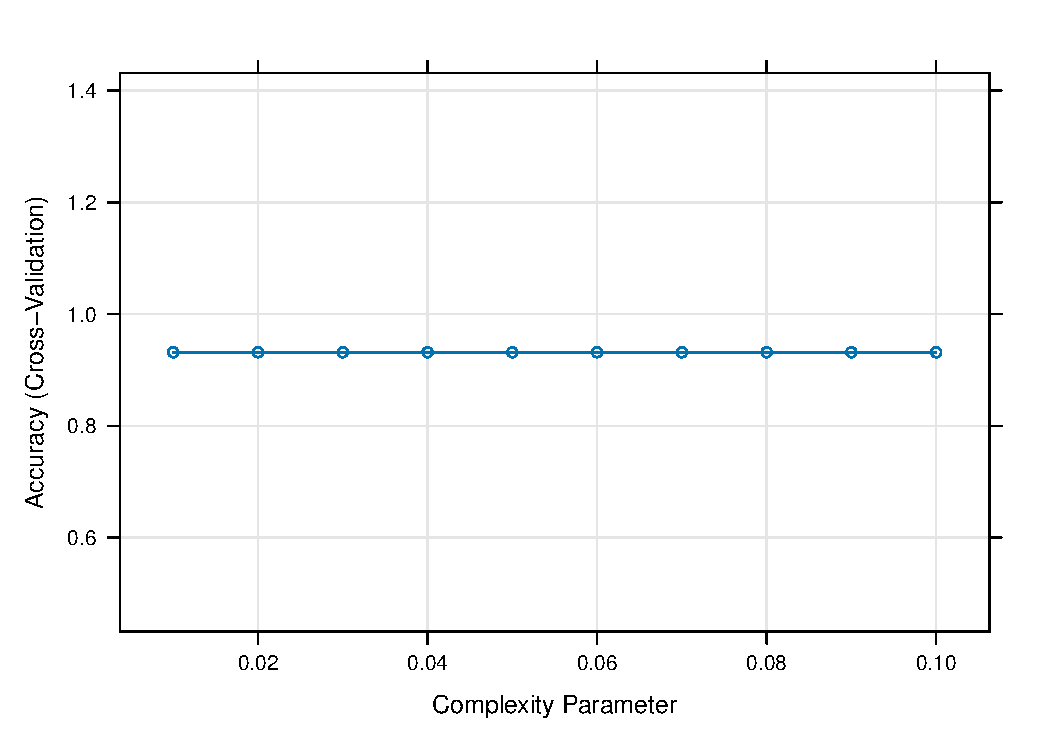
\includegraphics{37-t-SNE_files/figure-latex/unnamed-chunk-6-1.pdf}

\begin{Shaded}
\begin{Highlighting}[]
\NormalTok{p2}
\end{Highlighting}
\end{Shaded}

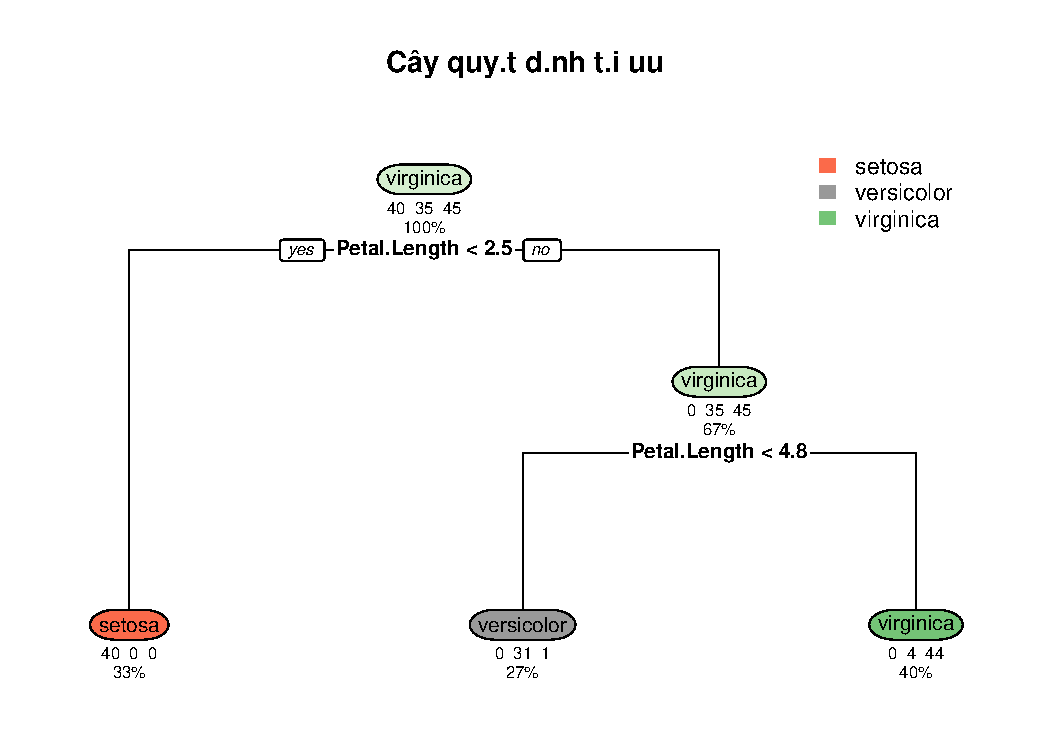
\includegraphics{37-t-SNE_files/figure-latex/unnamed-chunk-6-2.pdf}

\begin{Shaded}
\begin{Highlighting}[]
\NormalTok{p3}
\end{Highlighting}
\end{Shaded}

\includegraphics{37-t-SNE_files/figure-latex/unnamed-chunk-6-3.pdf}

Nhận xét: - t-SNE đã tạo ra một biểu diễn 2D cho dữ liệu mtcars, trong
đó các xe có đặc điểm tương tự thường nằm gần nhau - Có sự phân tách khá
rõ ràng giữa các loại động cơ, kiểu hộp số và số xi-lanh - Có thể thấy
xu hướng các xe có động cơ V-shaped thường nằm gần nhau, tương tự với
các xe có số xi-lanh giống nhau

\subsection{Khám phá ảnh hưởng của tham số
perplexity}\label{khuxe1m-phuxe1-ux1ea3nh-hux1b0ux1edfng-cux1ee7a-tham-sux1ed1-perplexity}

\begin{Shaded}
\begin{Highlighting}[]
\CommentTok{\# Tạo hàm để thực hiện t{-}SNE với perplexity khác nhau}
\NormalTok{run\_tsne }\OtherTok{\textless{}{-}} \ControlFlowTok{function}\NormalTok{(perplexity\_val) \{}
  \FunctionTok{set.seed}\NormalTok{(}\DecValTok{42}\NormalTok{)}
  \CommentTok{\# Sử dụng dữ liệu đã loại bỏ trùng lặp}
\NormalTok{  tsne }\OtherTok{\textless{}{-}} \FunctionTok{Rtsne}\NormalTok{(mtcars\_unique, }\AttributeTok{dims =} \DecValTok{2}\NormalTok{, }\AttributeTok{perplexity =}\NormalTok{ perplexity\_val, }
                \AttributeTok{verbose =} \ConstantTok{FALSE}\NormalTok{, }\AttributeTok{max\_iter =} \DecValTok{1000}\NormalTok{, }\AttributeTok{check\_duplicates =} \ConstantTok{FALSE}\NormalTok{)}
  
  \FunctionTok{data.frame}\NormalTok{(}
    \AttributeTok{x =}\NormalTok{ tsne}\SpecialCharTok{$}\NormalTok{Y[, }\DecValTok{1}\NormalTok{],}
    \AttributeTok{y =}\NormalTok{ tsne}\SpecialCharTok{$}\NormalTok{Y[, }\DecValTok{2}\NormalTok{],}
    \AttributeTok{cylinders =}\NormalTok{ cylinders\_unique,}
    \AttributeTok{perplexity =} \FunctionTok{as.factor}\NormalTok{(perplexity\_val)}
\NormalTok{  )}
\NormalTok{\}}

\CommentTok{\# Thực hiện t{-}SNE với các giá trị perplexity khác nhau}
\CommentTok{\# Perplexity không nên lớn hơn \textasciitilde{}n/3 với n là số điểm dữ liệu}
\NormalTok{max\_perplexity }\OtherTok{\textless{}{-}} \FunctionTok{floor}\NormalTok{(n\_samples}\SpecialCharTok{/}\DecValTok{3}\NormalTok{)}

\CommentTok{\# Chọn các giá trị perplexity phù hợp với kích thước dữ liệu}
\NormalTok{perplexity\_values }\OtherTok{\textless{}{-}} \FunctionTok{c}\NormalTok{(}\DecValTok{2}\NormalTok{, }\DecValTok{5}\NormalTok{, }\FunctionTok{min}\NormalTok{(}\DecValTok{10}\NormalTok{, max\_perplexity), }\FunctionTok{min}\NormalTok{(}\DecValTok{15}\NormalTok{, max\_perplexity))}
\NormalTok{perplexity\_values }\OtherTok{\textless{}{-}} \FunctionTok{unique}\NormalTok{(perplexity\_values) }\CommentTok{\# Loại bỏ giá trị trùng lặp nếu có}

\NormalTok{tsne\_results }\OtherTok{\textless{}{-}} \FunctionTok{do.call}\NormalTok{(rbind, }\FunctionTok{lapply}\NormalTok{(perplexity\_values, run\_tsne))}

\CommentTok{\# Vẽ biểu đồ so sánh}
\FunctionTok{ggplot}\NormalTok{(tsne\_results, }\FunctionTok{aes}\NormalTok{(}\AttributeTok{x =}\NormalTok{ x, }\AttributeTok{y =}\NormalTok{ y, }\AttributeTok{color =}\NormalTok{ cylinders)) }\SpecialCharTok{+}
  \FunctionTok{geom\_point}\NormalTok{(}\AttributeTok{size =} \DecValTok{3}\NormalTok{, }\AttributeTok{alpha =} \FloatTok{0.8}\NormalTok{) }\SpecialCharTok{+}
  \FunctionTok{scale\_color\_viridis\_d}\NormalTok{() }\SpecialCharTok{+}
  \FunctionTok{facet\_wrap}\NormalTok{(}\SpecialCharTok{\textasciitilde{}}\NormalTok{perplexity, }\AttributeTok{scales =} \StringTok{"free"}\NormalTok{) }\SpecialCharTok{+}
  \FunctionTok{labs}\NormalTok{(}\AttributeTok{title =} \StringTok{"Effect of perplexity parameter on t{-}SNE visualization"}\NormalTok{,}
       \AttributeTok{x =} \StringTok{"t{-}SNE dimension 1"}\NormalTok{,}
       \AttributeTok{y =} \StringTok{"t{-}SNE dimension 2"}\NormalTok{) }\SpecialCharTok{+}
  \FunctionTok{theme\_minimal}\NormalTok{()}
\end{Highlighting}
\end{Shaded}

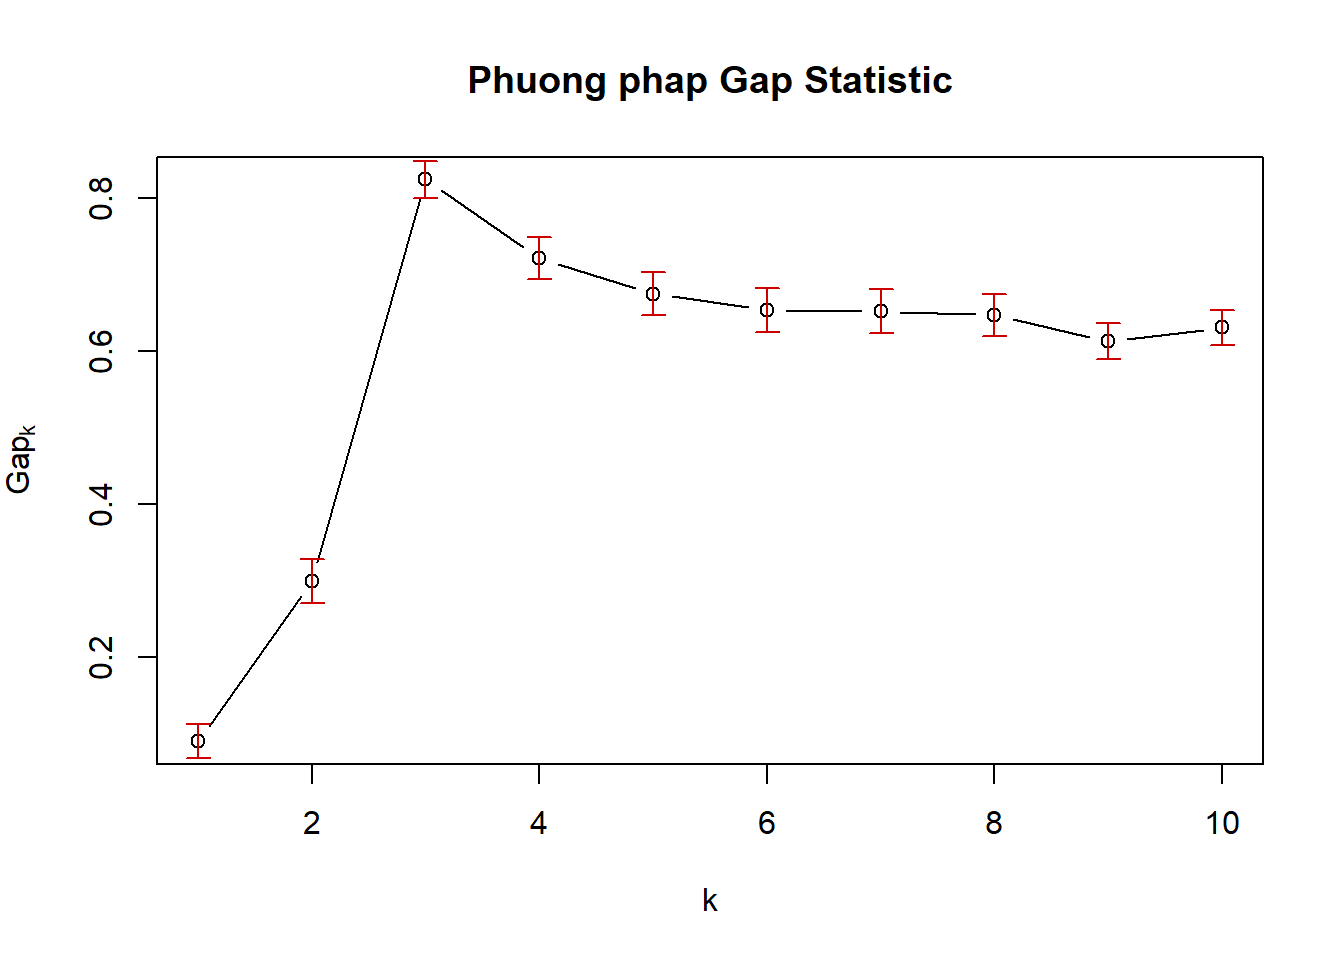
\includegraphics{37-t-SNE_files/figure-latex/unnamed-chunk-7-1.pdf}

Nhận xét về ảnh hưởng của perplexity: - Perplexity thấp (2-5): Tập trung
vào cấu trúc cục bộ, có thể tạo ra nhiều cụm nhỏ - Perplexity cao
(10-15): Tập trung vào cấu trúc toàn cục, các cụm có xu hướng gộp lại -
Với tập dữ liệu nhỏ như mtcars, perplexity không nên quá cao (không quá
1/3 số mẫu)

\section{So sánh t-SNE với PCA}\label{so-suxe1nh-t-sne-vux1edbi-pca}

\subsection{Thực hiện PCA}\label{thux1ef1c-hiux1ec7n-pca}

\begin{Shaded}
\begin{Highlighting}[]
\CommentTok{\# Thực hiện PCA trên cùng bộ dữ liệu mtcars}
\NormalTok{pca\_result }\OtherTok{\textless{}{-}} \FunctionTok{prcomp}\NormalTok{(mtcars\_unique, }\AttributeTok{center =} \ConstantTok{TRUE}\NormalTok{, }\AttributeTok{scale. =} \ConstantTok{TRUE}\NormalTok{)}

\CommentTok{\# Tạo dataframe với kết quả PCA và nhãn}
\NormalTok{pca\_df }\OtherTok{\textless{}{-}} \FunctionTok{data.frame}\NormalTok{(}
  \AttributeTok{x =}\NormalTok{ pca\_result}\SpecialCharTok{$}\NormalTok{x[, }\DecValTok{1}\NormalTok{],}
  \AttributeTok{y =}\NormalTok{ pca\_result}\SpecialCharTok{$}\NormalTok{x[, }\DecValTok{2}\NormalTok{],}
  \AttributeTok{engine\_type =}\NormalTok{ engine\_type\_unique,}
  \AttributeTok{transmission =}\NormalTok{ transmission\_unique,}
  \AttributeTok{cylinders =}\NormalTok{ cylinders\_unique,}
  \AttributeTok{car =}\NormalTok{ car\_names\_unique}
\NormalTok{)}

\CommentTok{\# Xem tóm tắt kết quả PCA}
\FunctionTok{summary}\NormalTok{(pca\_result)}
\end{Highlighting}
\end{Shaded}

\begin{verbatim}
## Importance of components:
##                           PC1    PC2     PC3     PC4     PC5     PC6     PC7
## Standard deviation     2.3782 1.4429 0.71008 0.51481 0.42797 0.35184 0.32413
## Proportion of Variance 0.6284 0.2313 0.05602 0.02945 0.02035 0.01375 0.01167
## Cumulative Proportion  0.6284 0.8598 0.91581 0.94525 0.96560 0.97936 0.99103
##                           PC8     PC9
## Standard deviation     0.2419 0.14896
## Proportion of Variance 0.0065 0.00247
## Cumulative Proportion  0.9975 1.00000
\end{verbatim}

\subsection{Phân tích các thành phần
chính}\label{phuxe2n-tuxedch-cuxe1c-thuxe0nh-phux1ea7n-chuxednh}

\begin{Shaded}
\begin{Highlighting}[]
\CommentTok{\# Biplot phân tích các biến đóng góp vào PCA}
\FunctionTok{fviz\_pca\_biplot}\NormalTok{(pca\_result, }
                \AttributeTok{label =} \StringTok{"var"}\NormalTok{,}
                \AttributeTok{col.ind =} \StringTok{"cos2"}\NormalTok{,}
                \AttributeTok{gradient.cols =} \FunctionTok{c}\NormalTok{(}\StringTok{"\#00AFBB"}\NormalTok{, }\StringTok{"\#E7B800"}\NormalTok{, }\StringTok{"\#FC4E07"}\NormalTok{),}
                \AttributeTok{repel =} \ConstantTok{TRUE}\NormalTok{,}
                \AttributeTok{title =} \StringTok{"PCA Biplot: Bien va quan sat"}\NormalTok{)}
\end{Highlighting}
\end{Shaded}

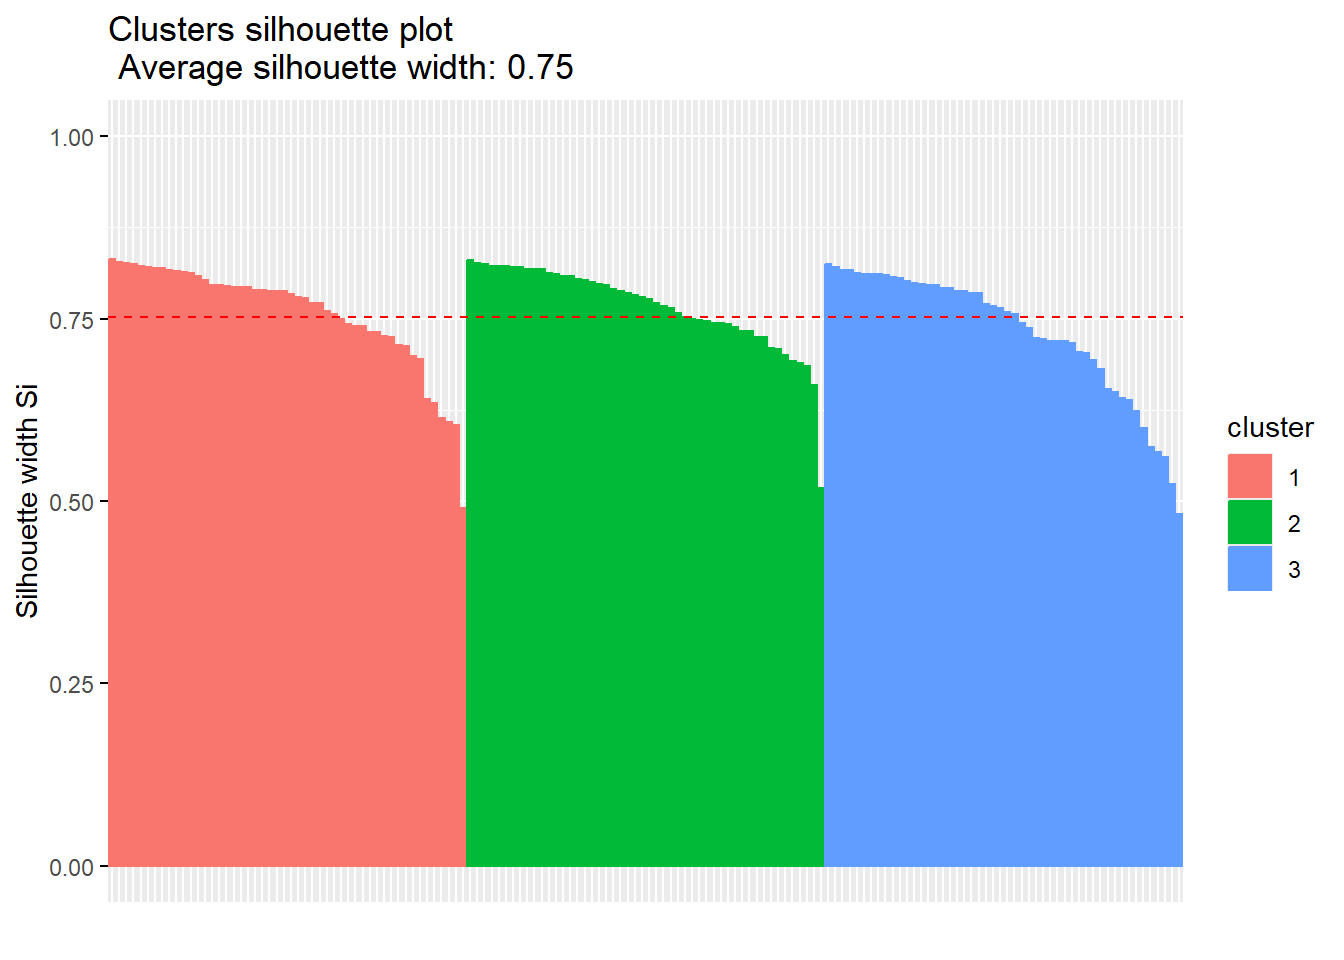
\includegraphics{37-t-SNE_files/figure-latex/unnamed-chunk-9-1.pdf}

\begin{Shaded}
\begin{Highlighting}[]
\CommentTok{\# Phân tích đóng góp của các biến vào PC1 và PC2}
\NormalTok{p1 }\OtherTok{\textless{}{-}} \FunctionTok{fviz\_contrib}\NormalTok{(pca\_result, }\AttributeTok{choice =} \StringTok{"var"}\NormalTok{, }\AttributeTok{axes =} \DecValTok{1}\NormalTok{, }\AttributeTok{top =} \DecValTok{10}\NormalTok{)}
\NormalTok{p2 }\OtherTok{\textless{}{-}} \FunctionTok{fviz\_contrib}\NormalTok{(pca\_result, }\AttributeTok{choice =} \StringTok{"var"}\NormalTok{, }\AttributeTok{axes =} \DecValTok{2}\NormalTok{, }\AttributeTok{top =} \DecValTok{10}\NormalTok{)}
\NormalTok{gridExtra}\SpecialCharTok{::}\FunctionTok{grid.arrange}\NormalTok{(p1, p2, }\AttributeTok{ncol =} \DecValTok{2}\NormalTok{)}
\end{Highlighting}
\end{Shaded}

\includegraphics{37-t-SNE_files/figure-latex/unnamed-chunk-9-2.pdf}

\subsection{So sánh trực quan giữa PCA và
t-SNE}\label{so-suxe1nh-trux1ef1c-quan-giux1eefa-pca-vuxe0-t-sne}

\begin{Shaded}
\begin{Highlighting}[]
\CommentTok{\# Vẽ biểu đồ PCA theo kiểu động cơ}
\NormalTok{pca\_plot1 }\OtherTok{\textless{}{-}} \FunctionTok{ggplot}\NormalTok{(pca\_df, }\FunctionTok{aes}\NormalTok{(}\AttributeTok{x =}\NormalTok{ x, }\AttributeTok{y =}\NormalTok{ y, }\AttributeTok{color =}\NormalTok{ engine\_type)) }\SpecialCharTok{+}
  \FunctionTok{geom\_point}\NormalTok{(}\AttributeTok{size =} \DecValTok{3}\NormalTok{, }\AttributeTok{alpha =} \FloatTok{0.8}\NormalTok{) }\SpecialCharTok{+}
  \FunctionTok{scale\_color\_viridis\_d}\NormalTok{() }\SpecialCharTok{+}
  \FunctionTok{labs}\NormalTok{(}\AttributeTok{title =} \StringTok{"PCA by Engine Type"}\NormalTok{,}
       \AttributeTok{x =} \StringTok{"PC1"}\NormalTok{,}
       \AttributeTok{y =} \StringTok{"PC2"}\NormalTok{,}
       \AttributeTok{color =} \StringTok{"Engine Type"}\NormalTok{) }\SpecialCharTok{+}
  \FunctionTok{theme\_minimal}\NormalTok{()}

\CommentTok{\# Vẽ biểu đồ t{-}SNE theo kiểu động cơ}
\NormalTok{tsne\_plot1 }\OtherTok{\textless{}{-}} \FunctionTok{ggplot}\NormalTok{(tsne\_df, }\FunctionTok{aes}\NormalTok{(}\AttributeTok{x =}\NormalTok{ x, }\AttributeTok{y =}\NormalTok{ y, }\AttributeTok{color =}\NormalTok{ engine\_type)) }\SpecialCharTok{+}
  \FunctionTok{geom\_point}\NormalTok{(}\AttributeTok{size =} \DecValTok{3}\NormalTok{, }\AttributeTok{alpha =} \FloatTok{0.8}\NormalTok{) }\SpecialCharTok{+}
  \FunctionTok{scale\_color\_viridis\_d}\NormalTok{() }\SpecialCharTok{+}
  \FunctionTok{labs}\NormalTok{(}\AttributeTok{title =} \StringTok{"t{-}SNE by Engine Type"}\NormalTok{,}
       \AttributeTok{x =} \StringTok{"t{-}SNE 1"}\NormalTok{,}
       \AttributeTok{y =} \StringTok{"t{-}SNE 2"}\NormalTok{,}
       \AttributeTok{color =} \StringTok{"Engine Type"}\NormalTok{) }\SpecialCharTok{+}
  \FunctionTok{theme\_minimal}\NormalTok{()}

\CommentTok{\# Hiển thị so sánh theo kiểu động cơ}
\NormalTok{gridExtra}\SpecialCharTok{::}\FunctionTok{grid.arrange}\NormalTok{(pca\_plot1, tsne\_plot1, }\AttributeTok{ncol =} \DecValTok{2}\NormalTok{)}
\end{Highlighting}
\end{Shaded}

\includegraphics{37-t-SNE_files/figure-latex/unnamed-chunk-10-1.pdf}

\begin{Shaded}
\begin{Highlighting}[]
\CommentTok{\# Vẽ biểu đồ PCA theo số xi{-}lanh}
\NormalTok{pca\_plot2 }\OtherTok{\textless{}{-}} \FunctionTok{ggplot}\NormalTok{(pca\_df, }\FunctionTok{aes}\NormalTok{(}\AttributeTok{x =}\NormalTok{ x, }\AttributeTok{y =}\NormalTok{ y, }\AttributeTok{color =}\NormalTok{ cylinders)) }\SpecialCharTok{+}
  \FunctionTok{geom\_point}\NormalTok{(}\AttributeTok{size =} \DecValTok{3}\NormalTok{, }\AttributeTok{alpha =} \FloatTok{0.8}\NormalTok{) }\SpecialCharTok{+}
  \FunctionTok{scale\_color\_viridis\_d}\NormalTok{(}\AttributeTok{option =} \StringTok{"inferno"}\NormalTok{) }\SpecialCharTok{+}
  \FunctionTok{labs}\NormalTok{(}\AttributeTok{title =} \StringTok{"PCA by Cylinders"}\NormalTok{,}
       \AttributeTok{x =} \StringTok{"PC1"}\NormalTok{,}
       \AttributeTok{y =} \StringTok{"PC2"}\NormalTok{,}
       \AttributeTok{color =} \StringTok{"Cylinders"}\NormalTok{) }\SpecialCharTok{+}
  \FunctionTok{theme\_minimal}\NormalTok{()}

\CommentTok{\# Vẽ biểu đồ t{-}SNE theo số xi{-}lanh}
\NormalTok{tsne\_plot2 }\OtherTok{\textless{}{-}} \FunctionTok{ggplot}\NormalTok{(tsne\_df, }\FunctionTok{aes}\NormalTok{(}\AttributeTok{x =}\NormalTok{ x, }\AttributeTok{y =}\NormalTok{ y, }\AttributeTok{color =}\NormalTok{ cylinders)) }\SpecialCharTok{+}
  \FunctionTok{geom\_point}\NormalTok{(}\AttributeTok{size =} \DecValTok{3}\NormalTok{, }\AttributeTok{alpha =} \FloatTok{0.8}\NormalTok{) }\SpecialCharTok{+}
  \FunctionTok{scale\_color\_viridis\_d}\NormalTok{(}\AttributeTok{option =} \StringTok{"inferno"}\NormalTok{) }\SpecialCharTok{+}
  \FunctionTok{labs}\NormalTok{(}\AttributeTok{title =} \StringTok{"t{-}SNE by Cylinders"}\NormalTok{,}
       \AttributeTok{x =} \StringTok{"t{-}SNE 1"}\NormalTok{,}
       \AttributeTok{y =} \StringTok{"t{-}SNE 2"}\NormalTok{,}
       \AttributeTok{color =} \StringTok{"Cylinders"}\NormalTok{) }\SpecialCharTok{+}
  \FunctionTok{theme\_minimal}\NormalTok{()}

\CommentTok{\# Hiển thị so sánh theo số xi{-}lanh}
\NormalTok{gridExtra}\SpecialCharTok{::}\FunctionTok{grid.arrange}\NormalTok{(pca\_plot2, tsne\_plot2, }\AttributeTok{ncol =} \DecValTok{2}\NormalTok{)}
\end{Highlighting}
\end{Shaded}

\includegraphics{37-t-SNE_files/figure-latex/unnamed-chunk-10-2.pdf}

Nhận xét khi so sánh PCA và t-SNE trên bộ dữ liệu mtcars:

\begin{itemize}
\tightlist
\item
  PCA là phương pháp tuyến tính tối đa hóa phương sai, cho phép chúng ta
  hiểu được đóng góp của các biến gốc
\item
  t-SNE là phương pháp phi tuyến tính tập trung vào bảo toàn cấu trúc
  cục bộ
\item
  Trong PCA, chúng ta thấy PC1 giải thích khoảng 60\% phương sai, và chủ
  yếu liên quan đến các biến về kích thước động cơ (disp, cyl) và hiệu
  suất (hp, mpg)
\item
  t-SNE có xu hướng tạo ra các cụm rõ ràng hơn, đặc biệt cho các nhóm xe
  có số xi-lanh giống nhau
\item
  Cả hai phương pháp đều cho thấy sự phân tách giữa các nhóm xe, nhưng
  t-SNE có thể làm nổi bật các mẫu cục bộ mà PCA có thể bỏ qua
\item
  PCA có ưu điểm là nhanh hơn, có thể áp dụng cho dữ liệu mới, và giúp
  hiểu cấu trúc dữ liệu gốc thông qua loadings
\item
  t-SNE thường tốt hơn cho mục đích trực quan hóa và khám phá dữ liệu,
  nhưng không thể hiện được đóng góp của các biến gốc
\end{itemize}

số viết tay).

\subsection{Phân tích bộ dữ liệu USArrests với
t-SNE}\label{phuxe2n-tuxedch-bux1ed9-dux1eef-liux1ec7u-usarrests-vux1edbi-t-sne}

\begin{Shaded}
\begin{Highlighting}[]
\CommentTok{\# Tải bộ dữ liệu USArrests}
\FunctionTok{data}\NormalTok{(USArrests)}

\CommentTok{\# Xem cấu trúc và thông tin cơ bản}
\FunctionTok{str}\NormalTok{(USArrests)}
\end{Highlighting}
\end{Shaded}

\begin{verbatim}
## 'data.frame':    50 obs. of  4 variables:
##  $ Murder  : num  13.2 10 8.1 8.8 9 7.9 3.3 5.9 15.4 17.4 ...
##  $ Assault : int  236 263 294 190 276 204 110 238 335 211 ...
##  $ UrbanPop: int  58 48 80 50 91 78 77 72 80 60 ...
##  $ Rape    : num  21.2 44.5 31 19.5 40.6 38.7 11.1 15.8 31.9 25.8 ...
\end{verbatim}

\begin{Shaded}
\begin{Highlighting}[]
\FunctionTok{head}\NormalTok{(USArrests)}
\end{Highlighting}
\end{Shaded}

\begin{verbatim}
##            Murder Assault UrbanPop Rape
## Alabama      13.2     236       58 21.2
## Alaska       10.0     263       48 44.5
## Arizona       8.1     294       80 31.0
## Arkansas      8.8     190       50 19.5
## California    9.0     276       91 40.6
## Colorado      7.9     204       78 38.7
\end{verbatim}

\begin{Shaded}
\begin{Highlighting}[]
\CommentTok{\# Tóm tắt thống kê}
\FunctionTok{summary}\NormalTok{(USArrests)}
\end{Highlighting}
\end{Shaded}

\begin{verbatim}
##      Murder          Assault         UrbanPop          Rape      
##  Min.   : 0.800   Min.   : 45.0   Min.   :32.00   Min.   : 7.30  
##  1st Qu.: 4.075   1st Qu.:109.0   1st Qu.:54.50   1st Qu.:15.07  
##  Median : 7.250   Median :159.0   Median :66.00   Median :20.10  
##  Mean   : 7.788   Mean   :170.8   Mean   :65.54   Mean   :21.23  
##  3rd Qu.:11.250   3rd Qu.:249.0   3rd Qu.:77.75   3rd Qu.:26.18  
##  Max.   :17.400   Max.   :337.0   Max.   :91.00   Max.   :46.00
\end{verbatim}

Bộ dữ liệu USArrests chứa thông tin về tỷ lệ tội phạm cho 50 bang của
Hoa Kỳ vào năm 1973 với các biến: - Murder: Số vụ giết người trên
100,000 dân - Assault: Số vụ hành hung trên 100,000 dân - UrbanPop: Tỷ
lệ dân số đô thị (\%) - Rape: Số vụ hiếp dâm trên 100,000 dân

\begin{Shaded}
\begin{Highlighting}[]
\CommentTok{\# Chuẩn bị dữ liệu}
\NormalTok{state\_names }\OtherTok{\textless{}{-}} \FunctionTok{rownames}\NormalTok{(USArrests)}
\NormalTok{arrests\_data }\OtherTok{\textless{}{-}}\NormalTok{ USArrests}

\CommentTok{\# Chuẩn hóa dữ liệu}
\NormalTok{arrests\_scaled }\OtherTok{\textless{}{-}} \FunctionTok{scale}\NormalTok{(arrests\_data)}

\CommentTok{\# Kiểm tra điểm trùng lặp}
\NormalTok{arrests\_duplicates }\OtherTok{\textless{}{-}} \FunctionTok{duplicated}\NormalTok{(arrests\_scaled)}
\FunctionTok{cat}\NormalTok{(}\StringTok{"Số bang trùng lặp:"}\NormalTok{, }\FunctionTok{sum}\NormalTok{(arrests\_duplicates), }\StringTok{"}\SpecialCharTok{\textbackslash{}n}\StringTok{"}\NormalTok{)}
\end{Highlighting}
\end{Shaded}

\begin{verbatim}
## Số bang trùng lặp: 0
\end{verbatim}

\begin{Shaded}
\begin{Highlighting}[]
\CommentTok{\# Nếu có điểm trùng lặp, loại bỏ chúng}
\NormalTok{arrests\_unique }\OtherTok{\textless{}{-}}\NormalTok{ arrests\_scaled[}\SpecialCharTok{!}\NormalTok{arrests\_duplicates, ]}
\NormalTok{state\_names\_unique }\OtherTok{\textless{}{-}}\NormalTok{ state\_names[}\SpecialCharTok{!}\NormalTok{arrests\_duplicates]}

\CommentTok{\# Thực hiện t{-}SNE}
\FunctionTok{set.seed}\NormalTok{(}\DecValTok{42}\NormalTok{)}
\CommentTok{\# Chọn perplexity phù hợp (không quá lớn so với số mẫu)}
\NormalTok{perplexity\_val }\OtherTok{\textless{}{-}} \FunctionTok{min}\NormalTok{(}\DecValTok{15}\NormalTok{, }\FunctionTok{floor}\NormalTok{(}\FunctionTok{nrow}\NormalTok{(arrests\_unique)}\SpecialCharTok{/}\DecValTok{3}\NormalTok{))}
\NormalTok{arrests\_tsne }\OtherTok{\textless{}{-}} \FunctionTok{Rtsne}\NormalTok{(arrests\_unique, }\AttributeTok{dims =} \DecValTok{2}\NormalTok{, }\AttributeTok{perplexity =}\NormalTok{ perplexity\_val, }
                     \AttributeTok{verbose =} \ConstantTok{TRUE}\NormalTok{, }\AttributeTok{max\_iter =} \DecValTok{1000}\NormalTok{, }\AttributeTok{check\_duplicates =} \ConstantTok{FALSE}\NormalTok{)}
\end{Highlighting}
\end{Shaded}

\begin{verbatim}
## Performing PCA
## Read the 50 x 4 data matrix successfully!
## OpenMP is working. 1 threads.
## Using no_dims = 2, perplexity = 15.000000, and theta = 0.500000
## Computing input similarities...
## Building tree...
## Done in 0.01 seconds (sparsity = 0.964800)!
## Learning embedding...
## Iteration 50: error is 60.530003 (50 iterations in 0.01 seconds)
## Iteration 100: error is 52.597460 (50 iterations in 0.01 seconds)
## Iteration 150: error is 53.156755 (50 iterations in 0.01 seconds)
## Iteration 200: error is 52.316403 (50 iterations in 0.01 seconds)
## Iteration 250: error is 52.461066 (50 iterations in 0.01 seconds)
## Iteration 300: error is 1.628035 (50 iterations in 0.00 seconds)
## Iteration 350: error is 1.237180 (50 iterations in 0.00 seconds)
## Iteration 400: error is 0.747900 (50 iterations in 0.00 seconds)
## Iteration 450: error is 0.600039 (50 iterations in 0.00 seconds)
## Iteration 500: error is 0.534821 (50 iterations in 0.00 seconds)
## Iteration 550: error is 0.415982 (50 iterations in 0.00 seconds)
## Iteration 600: error is 0.366624 (50 iterations in 0.00 seconds)
## Iteration 650: error is 0.351396 (50 iterations in 0.00 seconds)
## Iteration 700: error is 0.219800 (50 iterations in 0.00 seconds)
## Iteration 750: error is 0.195022 (50 iterations in 0.00 seconds)
## Iteration 800: error is 0.184900 (50 iterations in 0.00 seconds)
## Iteration 850: error is 0.172711 (50 iterations in 0.00 seconds)
## Iteration 900: error is 0.170133 (50 iterations in 0.01 seconds)
## Iteration 950: error is 0.163149 (50 iterations in 0.01 seconds)
## Iteration 1000: error is 0.167233 (50 iterations in 0.01 seconds)
## Fitting performed in 0.11 seconds.
\end{verbatim}

\begin{Shaded}
\begin{Highlighting}[]
\CommentTok{\# Tạo dataframe với kết quả}
\NormalTok{arrests\_tsne\_df }\OtherTok{\textless{}{-}} \FunctionTok{data.frame}\NormalTok{(}
  \AttributeTok{x =}\NormalTok{ arrests\_tsne}\SpecialCharTok{$}\NormalTok{Y[, }\DecValTok{1}\NormalTok{],}
  \AttributeTok{y =}\NormalTok{ arrests\_tsne}\SpecialCharTok{$}\NormalTok{Y[, }\DecValTok{2}\NormalTok{],}
  \AttributeTok{state =}\NormalTok{ state\_names\_unique}
\NormalTok{)}

\CommentTok{\# Kết hợp dữ liệu gốc với kết quả t{-}SNE}
\NormalTok{arrests\_tsne\_df }\OtherTok{\textless{}{-}} \FunctionTok{cbind}\NormalTok{(arrests\_tsne\_df, arrests\_data[}\SpecialCharTok{!}\NormalTok{arrests\_duplicates, ])}

\CommentTok{\# Thêm thông tin vùng địa lý}
\CommentTok{\# Phân chia các bang theo vùng (chỉ là ví dụ, có thể điều chỉnh)}
\NormalTok{northeast }\OtherTok{\textless{}{-}} \FunctionTok{c}\NormalTok{(}\StringTok{"Maine"}\NormalTok{, }\StringTok{"New Hampshire"}\NormalTok{, }\StringTok{"Vermont"}\NormalTok{, }\StringTok{"Massachusetts"}\NormalTok{, }\StringTok{"Rhode Island"}\NormalTok{, }
               \StringTok{"Connecticut"}\NormalTok{, }\StringTok{"New York"}\NormalTok{, }\StringTok{"New Jersey"}\NormalTok{, }\StringTok{"Pennsylvania"}\NormalTok{)}
\NormalTok{midwest }\OtherTok{\textless{}{-}} \FunctionTok{c}\NormalTok{(}\StringTok{"Ohio"}\NormalTok{, }\StringTok{"Indiana"}\NormalTok{, }\StringTok{"Illinois"}\NormalTok{, }\StringTok{"Michigan"}\NormalTok{, }\StringTok{"Wisconsin"}\NormalTok{, }
             \StringTok{"Minnesota"}\NormalTok{, }\StringTok{"Iowa"}\NormalTok{, }\StringTok{"Missouri"}\NormalTok{, }\StringTok{"North Dakota"}\NormalTok{, }\StringTok{"South Dakota"}\NormalTok{, }
             \StringTok{"Nebraska"}\NormalTok{, }\StringTok{"Kansas"}\NormalTok{)}
\NormalTok{south }\OtherTok{\textless{}{-}} \FunctionTok{c}\NormalTok{(}\StringTok{"Delaware"}\NormalTok{, }\StringTok{"Maryland"}\NormalTok{, }\StringTok{"Virginia"}\NormalTok{, }\StringTok{"West Virginia"}\NormalTok{, }\StringTok{"North Carolina"}\NormalTok{,}
           \StringTok{"South Carolina"}\NormalTok{, }\StringTok{"Georgia"}\NormalTok{, }\StringTok{"Florida"}\NormalTok{, }\StringTok{"Kentucky"}\NormalTok{, }\StringTok{"Tennessee"}\NormalTok{, }
           \StringTok{"Alabama"}\NormalTok{, }\StringTok{"Mississippi"}\NormalTok{, }\StringTok{"Arkansas"}\NormalTok{, }\StringTok{"Louisiana"}\NormalTok{, }\StringTok{"Oklahoma"}\NormalTok{, }\StringTok{"Texas"}\NormalTok{)}
\NormalTok{west }\OtherTok{\textless{}{-}} \FunctionTok{c}\NormalTok{(}\StringTok{"Montana"}\NormalTok{, }\StringTok{"Idaho"}\NormalTok{, }\StringTok{"Wyoming"}\NormalTok{, }\StringTok{"Colorado"}\NormalTok{, }\StringTok{"New Mexico"}\NormalTok{, }\StringTok{"Arizona"}\NormalTok{, }\StringTok{"Utah"}\NormalTok{,}
          \StringTok{"Nevada"}\NormalTok{, }\StringTok{"Washington"}\NormalTok{, }\StringTok{"Oregon"}\NormalTok{, }\StringTok{"California"}\NormalTok{, }\StringTok{"Alaska"}\NormalTok{, }\StringTok{"Hawaii"}\NormalTok{)}

\CommentTok{\# Thêm cột vùng}
\NormalTok{arrests\_tsne\_df}\SpecialCharTok{$}\NormalTok{region }\OtherTok{\textless{}{-}} \ConstantTok{NA}
\NormalTok{arrests\_tsne\_df}\SpecialCharTok{$}\NormalTok{region[arrests\_tsne\_df}\SpecialCharTok{$}\NormalTok{state }\SpecialCharTok{\%in\%}\NormalTok{ northeast] }\OtherTok{\textless{}{-}} \StringTok{"Northeast"}
\NormalTok{arrests\_tsne\_df}\SpecialCharTok{$}\NormalTok{region[arrests\_tsne\_df}\SpecialCharTok{$}\NormalTok{state }\SpecialCharTok{\%in\%}\NormalTok{ midwest] }\OtherTok{\textless{}{-}} \StringTok{"Midwest"}
\NormalTok{arrests\_tsne\_df}\SpecialCharTok{$}\NormalTok{region[arrests\_tsne\_df}\SpecialCharTok{$}\NormalTok{state }\SpecialCharTok{\%in\%}\NormalTok{ south] }\OtherTok{\textless{}{-}} \StringTok{"South"}
\NormalTok{arrests\_tsne\_df}\SpecialCharTok{$}\NormalTok{region[arrests\_tsne\_df}\SpecialCharTok{$}\NormalTok{state }\SpecialCharTok{\%in\%}\NormalTok{ west] }\OtherTok{\textless{}{-}} \StringTok{"West"}
\NormalTok{arrests\_tsne\_df}\SpecialCharTok{$}\NormalTok{region }\OtherTok{\textless{}{-}} \FunctionTok{factor}\NormalTok{(arrests\_tsne\_df}\SpecialCharTok{$}\NormalTok{region)}
\end{Highlighting}
\end{Shaded}

\subsection{Trực quan hóa kết quả t-SNE trên
USArrests}\label{trux1ef1c-quan-huxf3a-kux1ebft-quux1ea3-t-sne-truxean-usarrests}

\begin{Shaded}
\begin{Highlighting}[]
\CommentTok{\# Vẽ biểu đồ t{-}SNE cho USArrests theo vùng địa lý}
\NormalTok{p1 }\OtherTok{\textless{}{-}} \FunctionTok{ggplot}\NormalTok{(arrests\_tsne\_df, }\FunctionTok{aes}\NormalTok{(}\AttributeTok{x =}\NormalTok{ x, }\AttributeTok{y =}\NormalTok{ y, }\AttributeTok{color =}\NormalTok{ region)) }\SpecialCharTok{+}
  \FunctionTok{geom\_point}\NormalTok{(}\AttributeTok{size =} \DecValTok{3}\NormalTok{, }\AttributeTok{alpha =} \FloatTok{0.8}\NormalTok{) }\SpecialCharTok{+}
  \FunctionTok{geom\_text}\NormalTok{(}\FunctionTok{aes}\NormalTok{(}\AttributeTok{label =}\NormalTok{ state), }\AttributeTok{vjust =} \SpecialCharTok{{-}}\FloatTok{0.5}\NormalTok{, }\AttributeTok{size =} \DecValTok{3}\NormalTok{, }\AttributeTok{check\_overlap =} \ConstantTok{TRUE}\NormalTok{) }\SpecialCharTok{+}
  \FunctionTok{scale\_color\_viridis\_d}\NormalTok{() }\SpecialCharTok{+}
  \FunctionTok{labs}\NormalTok{(}\AttributeTok{title =} \StringTok{"t{-}SNE visualization of US States by Crime Rates"}\NormalTok{,}
       \AttributeTok{subtitle =} \StringTok{"Colored by Geographic Region"}\NormalTok{,}
       \AttributeTok{x =} \StringTok{"t{-}SNE dimension 1"}\NormalTok{,}
       \AttributeTok{y =} \StringTok{"t{-}SNE dimension 2"}\NormalTok{) }\SpecialCharTok{+}
  \FunctionTok{theme\_minimal}\NormalTok{()}

\CommentTok{\# Vẽ biểu đồ theo tỷ lệ Murder}
\NormalTok{p2 }\OtherTok{\textless{}{-}} \FunctionTok{ggplot}\NormalTok{(arrests\_tsne\_df, }\FunctionTok{aes}\NormalTok{(}\AttributeTok{x =}\NormalTok{ x, }\AttributeTok{y =}\NormalTok{ y, }\AttributeTok{color =}\NormalTok{ Murder)) }\SpecialCharTok{+}
  \FunctionTok{geom\_point}\NormalTok{(}\AttributeTok{size =} \DecValTok{3}\NormalTok{, }\AttributeTok{alpha =} \FloatTok{0.8}\NormalTok{) }\SpecialCharTok{+}
  \FunctionTok{geom\_text}\NormalTok{(}\FunctionTok{aes}\NormalTok{(}\AttributeTok{label =}\NormalTok{ state), }\AttributeTok{vjust =} \SpecialCharTok{{-}}\FloatTok{0.5}\NormalTok{, }\AttributeTok{size =} \DecValTok{3}\NormalTok{, }\AttributeTok{check\_overlap =} \ConstantTok{TRUE}\NormalTok{) }\SpecialCharTok{+}
  \FunctionTok{scale\_color\_viridis\_c}\NormalTok{() }\SpecialCharTok{+}
  \FunctionTok{labs}\NormalTok{(}\AttributeTok{title =} \StringTok{"t{-}SNE visualization of US States by Crime Rates"}\NormalTok{,}
       \AttributeTok{subtitle =} \StringTok{"Colored by Murder Rate"}\NormalTok{,}
       \AttributeTok{x =} \StringTok{"t{-}SNE dimension 1"}\NormalTok{,}
       \AttributeTok{y =} \StringTok{"t{-}SNE dimension 2"}\NormalTok{) }\SpecialCharTok{+}
  \FunctionTok{theme\_minimal}\NormalTok{()}

\CommentTok{\# Hiển thị các biểu đồ}
\NormalTok{p1}
\end{Highlighting}
\end{Shaded}

\includegraphics{37-t-SNE_files/figure-latex/unnamed-chunk-13-1.pdf}

\begin{Shaded}
\begin{Highlighting}[]
\NormalTok{p2}
\end{Highlighting}
\end{Shaded}

\includegraphics{37-t-SNE_files/figure-latex/unnamed-chunk-13-2.pdf}

\begin{Shaded}
\begin{Highlighting}[]
\CommentTok{\# Vẽ biểu đồ theo tỷ lệ đô thị hóa}
\NormalTok{p3 }\OtherTok{\textless{}{-}} \FunctionTok{ggplot}\NormalTok{(arrests\_tsne\_df, }\FunctionTok{aes}\NormalTok{(}\AttributeTok{x =}\NormalTok{ x, }\AttributeTok{y =}\NormalTok{ y, }\AttributeTok{color =}\NormalTok{ UrbanPop)) }\SpecialCharTok{+}
  \FunctionTok{geom\_point}\NormalTok{(}\AttributeTok{size =} \DecValTok{3}\NormalTok{, }\AttributeTok{alpha =} \FloatTok{0.8}\NormalTok{) }\SpecialCharTok{+}
  \FunctionTok{geom\_text}\NormalTok{(}\FunctionTok{aes}\NormalTok{(}\AttributeTok{label =}\NormalTok{ state), }\AttributeTok{vjust =} \SpecialCharTok{{-}}\FloatTok{0.5}\NormalTok{, }\AttributeTok{size =} \DecValTok{3}\NormalTok{, }\AttributeTok{check\_overlap =} \ConstantTok{TRUE}\NormalTok{) }\SpecialCharTok{+}
  \FunctionTok{scale\_color\_viridis\_c}\NormalTok{(}\AttributeTok{option =} \StringTok{"plasma"}\NormalTok{) }\SpecialCharTok{+}
  \FunctionTok{labs}\NormalTok{(}\AttributeTok{title =} \StringTok{"t{-}SNE visualization of US States by Crime Rates"}\NormalTok{,}
       \AttributeTok{subtitle =} \StringTok{"Colored by Urban Population Percentage"}\NormalTok{,}
       \AttributeTok{x =} \StringTok{"t{-}SNE dimension 1"}\NormalTok{,}
       \AttributeTok{y =} \StringTok{"t{-}SNE dimension 2"}\NormalTok{) }\SpecialCharTok{+}
  \FunctionTok{theme\_minimal}\NormalTok{()}

\NormalTok{p3}
\end{Highlighting}
\end{Shaded}

\includegraphics{37-t-SNE_files/figure-latex/unnamed-chunk-13-3.pdf}

Nhận xét: - t-SNE đã tạo ra biểu diễn 2D của các bang dựa trên mẫu tội
phạm và tỷ lệ đô thị hóa - Có thể thấy các bang trong cùng một vùng địa
lý thường có xu hướng nằm gần nhau trên không gian t-SNE - Các bang có
tỷ lệ tội phạm tương tự nhau được nhóm lại với nhau - Biểu đồ màu theo
tỷ lệ Murder cho thấy các bang với tỷ lệ giết người cao (màu sáng)
thường tập trung ở một khu vực - Tỷ lệ đô thị hóa cũng cho thấy một mẫu
thú vị trong kết quả t-SNE

\section{Giảm chiều dữ liệu với t-SNE cho bài toán thực
tế}\label{giux1ea3m-chiux1ec1u-dux1eef-liux1ec7u-vux1edbi-t-sne-cho-buxe0i-touxe1n-thux1ef1c-tux1ebf}

\subsection{Ứng dụng t-SNE trong phân tích dữ liệu
lớn}\label{ux1ee9ng-dux1ee5ng-t-sne-trong-phuxe2n-tuxedch-dux1eef-liux1ec7u-lux1edbn}

Trong phần này, chúng ta sẽ thảo luận về cách t-SNE có thể được áp dụng
trong các bài toán thực tế với dữ liệu lớn.

\subsubsection{Quy trình xử lý dữ liệu lớn với
t-SNE}\label{quy-truxecnh-xux1eed-luxfd-dux1eef-liux1ec7u-lux1edbn-vux1edbi-t-sne}

Khi làm việc với dữ liệu có số chiều cao và kích thước lớn, quy trình
tiếp cận thường là:

\begin{enumerate}
\def\labelenumi{\arabic{enumi}.}
\tightlist
\item
  \textbf{Làm sạch và chuẩn hóa dữ liệu}

  \begin{itemize}
  \tightlist
  \item
    Xử lý giá trị thiếu, loại bỏ ngoại lai
  \item
    Chuẩn hóa các biến số
  \end{itemize}
\item
  \textbf{Giảm kích thước dữ liệu (nếu cần)}

  \begin{itemize}
  \tightlist
  \item
    Với dữ liệu rất lớn (hàng triệu mẫu), có thể lấy mẫu ngẫu nhiên
  \item
    Với dữ liệu có nhiều chiều (hàng nghìn biến), có thể dùng PCA trước
    để giảm xuống 50-100 chiều
  \end{itemize}
\item
  \textbf{Áp dụng t-SNE}

  \begin{itemize}
  \tightlist
  \item
    Chọn perplexity phù hợp với kích thước dữ liệu
  \item
    Thử nghiệm với nhiều giá trị tham số
  \item
    Đánh giá tính ổn định của kết quả
  \end{itemize}
\item
  \textbf{Giải thích và ứng dụng kết quả}

  \begin{itemize}
  \tightlist
  \item
    Kết hợp với các phương pháp phân cụm
  \item
    Sử dụng để trực quan hóa và khám phá dữ liệu
  \end{itemize}
\end{enumerate}

\subsubsection{Ví dụ về các bài toán thực
tế}\label{vuxed-dux1ee5-vux1ec1-cuxe1c-buxe0i-touxe1n-thux1ef1c-tux1ebf}

\begin{enumerate}
\def\labelenumi{\arabic{enumi}.}
\tightlist
\item
  \textbf{Phân tích dữ liệu gene và protein}

  \begin{itemize}
  \tightlist
  \item
    Giảm chiều dữ liệu biểu hiện gene (thường có hàng nghìn gene)
  \item
    Phát hiện nhóm tế bào có chức năng tương tự
  \end{itemize}
\item
  \textbf{Phân tích văn bản và xử lý ngôn ngữ tự nhiên}

  \begin{itemize}
  \tightlist
  \item
    Trực quan hóa không gian embedding của từ hoặc văn bản
  \item
    Phát hiện các chủ đề tương tự
  \end{itemize}
\item
  \textbf{Phát hiện gian lận và bất thường}

  \begin{itemize}
  \tightlist
  \item
    Giảm chiều các đặc trưng giao dịch
  \item
    Xác định các mẫu giao dịch bất thường
  \end{itemize}
\end{enumerate}

\subsection{Các khuyến nghị khi sử dụng
t-SNE}\label{cuxe1c-khuyux1ebfn-nghux1ecb-khi-sux1eed-dux1ee5ng-t-sne}

\begin{enumerate}
\def\labelenumi{\arabic{enumi}.}
\tightlist
\item
  \textbf{Tiền xử lý dữ liệu:}

  \begin{itemize}
  \tightlist
  \item
    Chuẩn hóa dữ liệu trước khi áp dụng t-SNE
  \item
    Loại bỏ các biến không liên quan hoặc nhiễu
  \item
    Với dữ liệu lớn, cân nhắc giảm chiều bằng PCA trước
  \end{itemize}
\item
  \textbf{Điều chỉnh tham số:}

  \begin{itemize}
  \tightlist
  \item
    \textbf{Perplexity}: Thử nghiệm với nhiều giá trị (5-50), không vượt
    quá 1/3 số mẫu
  \item
    \textbf{Số lần lặp}: Tăng số lần lặp (500-2000) nếu kết quả chưa hội
    tụ
  \item
    \textbf{Learning rate}: Điều chỉnh nếu kết quả không ổn định
  \end{itemize}
\item
  \textbf{Giải thích kết quả một cách thận trọng:}

  \begin{itemize}
  \tightlist
  \item
    Chỉ giải thích về khoảng cách tương đối giữa các điểm lân cận
  \item
    Không nên giải thích về kích thước của các cụm
  \item
    Khoảng cách giữa các cụm xa nhau không mang nhiều ý nghĩa
  \end{itemize}
\item
  \textbf{Đánh giá tính ổn định:}

  \begin{itemize}
  \tightlist
  \item
    Thực hiện t-SNE nhiều lần với các seed khác nhau
  \item
    So sánh kết quả giữa các lần chạy
  \end{itemize}
\end{enumerate}

\subsection{So sánh với các phương pháp giảm chiều
khác}\label{so-suxe1nh-vux1edbi-cuxe1c-phux1b0ux1a1ng-phuxe1p-giux1ea3m-chiux1ec1u-khuxe1c}

\begin{longtable}[]{@{}
  >{\raggedright\arraybackslash}p{(\columnwidth - 12\tabcolsep) * \real{0.1287}}
  >{\raggedright\arraybackslash}p{(\columnwidth - 12\tabcolsep) * \real{0.1188}}
  >{\raggedright\arraybackslash}p{(\columnwidth - 12\tabcolsep) * \real{0.1881}}
  >{\raggedright\arraybackslash}p{(\columnwidth - 12\tabcolsep) * \real{0.0792}}
  >{\raggedright\arraybackslash}p{(\columnwidth - 12\tabcolsep) * \real{0.1782}}
  >{\raggedright\arraybackslash}p{(\columnwidth - 12\tabcolsep) * \real{0.1485}}
  >{\raggedright\arraybackslash}p{(\columnwidth - 12\tabcolsep) * \real{0.1584}}@{}}
\toprule\noalign{}
\begin{minipage}[b]{\linewidth}\raggedright
Phương pháp
\end{minipage} & \begin{minipage}[b]{\linewidth}\raggedright
Tuyến tính
\end{minipage} & \begin{minipage}[b]{\linewidth}\raggedright
Bảo toàn cấu trúc
\end{minipage} & \begin{minipage}[b]{\linewidth}\raggedright
Tốc độ
\end{minipage} & \begin{minipage}[b]{\linewidth}\raggedright
Khả năng mở rộng
\end{minipage} & \begin{minipage}[b]{\linewidth}\raggedright
Dễ giải thích
\end{minipage} & \begin{minipage}[b]{\linewidth}\raggedright
Ứng dụng chính
\end{minipage} \\
\midrule\noalign{}
\endhead
\bottomrule\noalign{}
\endlastfoot
PCA & Có & Toàn cục & Nhanh & Tốt & Cao & Giảm chiều, xử lý đa cộng
tuyến \\
t-SNE & Không & Cục bộ & Chậm & Kém & Thấp & Trực quan hóa, phát hiện
cụm \\
UMAP & Không & Cục bộ \& Toàn cục & Nhanh hơn t-SNE & Tốt hơn t-SNE &
Trung bình & Trực quan hóa, phân cụm \\
LDA & Có & Phân biệt lớp & Nhanh & Tốt & Cao & Phân loại có giám sát \\
MDS & Tùy thuộc & Toàn cục & Trung bình & Trung bình & Trung bình & Trực
quan hóa, phân tích tương đồng \\
Autoencoder & Không & Tùy thuộc & Chậm (khi huấn luyện) & Tốt & Thấp &
Giảm chiều phi tuyến, phát hiện bất thường \\
\end{longtable}

\section{Một số lưu ý khi sử dụng
t-SNE}\label{mux1ed9t-sux1ed1-lux1b0u-uxfd-khi-sux1eed-dux1ee5ng-t-sne}

\subsection{Hướng dẫn thực
hành}\label{hux1b0ux1edbng-dux1eabn-thux1ef1c-huxe0nh}

\begin{enumerate}
\def\labelenumi{\arabic{enumi}.}
\tightlist
\item
  \textbf{Xử lý dữ liệu đầu vào:}

  \begin{itemize}
  \tightlist
  \item
    Chuẩn hóa dữ liệu trước khi áp dụng t-SNE
  \item
    Loại bỏ các điểm trùng lặp (t-SNE yêu cầu các điểm là duy nhất)
  \item
    Với tập dữ liệu lớn, có thể cân nhắc giảm chiều bằng PCA trước khi
    áp dụng t-SNE
  \end{itemize}
\item
  \textbf{Điều chỉnh tham số:}

  \begin{itemize}
  \tightlist
  \item
    \textbf{Perplexity}: Thường nên từ 5-50, không vượt quá 1/3 số lượng
    mẫu. Perplexity có thể hiểu như ``số lượng láng giềng hiệu quả'' mà
    mỗi điểm nên xem xét.
  \item
    \textbf{Số lần lặp (iterations)}: Thường cần 500-1000 lần lặp để hội
    tụ, có thể tăng thêm nếu cần.
  \item
    \textbf{Learning rate}: Mặc định thường hoạt động tốt, nhưng có thể
    điều chỉnh để tránh tối ưu cục bộ.
  \end{itemize}
\item
  \textbf{Giải thích kết quả:}

  \begin{itemize}
  \tightlist
  \item
    t-SNE chỉ bảo toàn khoảng cách tương đối giữa các điểm lân cận
  \item
    Kích thước của các cụm không mang ý nghĩa thống kê
  \item
    Khoảng cách giữa các cụm không nên được giải thích trực tiếp
  \item
    Để kiểm tra mức độ phù hợp của kết quả, nên thử với các giá trị
    perplexity khác nhau
  \end{itemize}
\end{enumerate}

\subsection{Mở rộng sang UMAP}\label{mux1edf-rux1ed9ng-sang-umap}

UMAP (Uniform Manifold Approximation and Projection) là một phương pháp
giảm chiều phi tuyến tính mới hơn t-SNE, với một số ưu điểm:

\begin{itemize}
\tightlist
\item
  Nhanh hơn t-SNE đáng kể
\item
  Bảo toàn tốt hơn cả cấu trúc cục bộ và toàn cục
\item
  Ít nhạy cảm với tham số hơn
\item
  Có thể áp dụng cho dữ liệu mới (ánh xạ tổng quát)
\end{itemize}

\begin{Shaded}
\begin{Highlighting}[]
\CommentTok{\# Cài đặt và sử dụng UMAP (Code chỉ để minh họa)}
\CommentTok{\# install.packages("umap")}
\CommentTok{\# library(umap)}
\CommentTok{\# umap\_result \textless{}{-} umap(mtcars\_scaled)}
\end{Highlighting}
\end{Shaded}

\section{Kết luận}\label{kux1ebft-luux1eadn}

t-SNE là một công cụ mạnh mẽ cho việc trực quan hóa dữ liệu đa chiều,
đặc biệt phù hợp khi cần phát hiện các mẫu và cụm trong dữ liệu. Phương
pháp này cho phép chúng ta:

\begin{enumerate}
\def\labelenumi{\arabic{enumi}.}
\tightlist
\item
  \textbf{Trực quan hóa dữ liệu nhiều chiều} trong không gian 2D hoặc 3D
  một cách hiệu quả
\item
  \textbf{Phát hiện cấu trúc cục bộ} và mẫu phức tạp trong dữ liệu
\item
  \textbf{Khám phá các nhóm tự nhiên} mà các phương pháp tuyến tính như
  PCA có thể bỏ qua
\end{enumerate}

Tuy nhiên, cần sử dụng t-SNE cẩn thận và hiểu rõ các hạn chế của nó:

\begin{enumerate}
\def\labelenumi{\arabic{enumi}.}
\tightlist
\item
  \textbf{Không bảo toàn khoảng cách toàn cục}
\item
  \textbf{Chi phí tính toán cao} với các tập dữ liệu lớn
\item
  \textbf{Kết quả phụ thuộc vào tham số}
\item
  \textbf{Không tạo ra ánh xạ tổng quát} cho dữ liệu mới
\end{enumerate}

Trong thực tế, t-SNE thường được sử dụng kết hợp với các kỹ thuật khác
như PCA để đạt được hiệu quả tốt nhất. Đối với các ứng dụng đòi hỏi hiệu
suất cao hoặc bảo toàn cấu trúc toàn cục tốt hơn, có thể cân nhắc sử
dụng các phương pháp mới hơn như UMAP.

\section{Tài liệu tham khảo}\label{tuxe0i-liux1ec7u-tham-khux1ea3o}

\begin{enumerate}
\def\labelenumi{\arabic{enumi}.}
\item
  Van der Maaten, L., \& Hinton, G. (2008). Visualizing data using
  t-SNE. Journal of machine learning research, 9(11).
\item
  Wattenberg, M., Viégas, F., \& Johnson, I. (2016). How to use t-SNE
  effectively. Distill, 1(10), e2.
\item
  Linderman, G. C., \& Steinerberger, S. (2019). Clustering with t-SNE,
  provably. SIAM Journal on Mathematics of Data Science, 1(2), 313-332.
\item
  McInnes, L., Healy, J., \& Melville, J. (2018). UMAP: Uniform manifold
  approximation and projection for dimension reduction. arXiv preprint
  arXiv:1802.03426.
\item
  \url{https://distill.pub/2016/misread-tsne/}
\end{enumerate}

\end{document}
